\documentclass[aspectratio=169]{beamer}

% VT presentation template (Madrid + miniframes + circles)
\usetheme{Madrid}
\useoutertheme{miniframes}
\useinnertheme{circles}

\usepackage[utf8]{inputenc}
\usepackage[T1]{fontenc}
\usepackage{palatino}
\usepackage[default]{opensans}
\usefonttheme{default}

\usepackage{graphicx}
\usepackage{booktabs}
\usepackage{amsmath}
\usepackage{tikz}
\usepackage{colortbl}
\usepackage{listings}
\usepackage{enumitem}
\usepackage{xcolor}

\usetikzlibrary{positioning, arrows.meta, shapes.geometric, calc}

% Speaker notes toggle
\ifdefined\SHOWNOTES
  \usepackage{pgfpages}
  \setbeameroption{show notes on second screen=right}
\fi

% Virginia Tech official colors (VT template)
\definecolor{myRed}{RGB}{134,31,65}       % VT Maroon
\definecolor{myOrange}{RGB}{229,117,31}   % VT Orange
% Legacy aliases kept so existing TikZ frames keep working
\colorlet{vtMaroon}{myRed}
\colorlet{vtOrange}{myOrange}
\colorlet{vtWhite}{white}
\colorlet{mTeal}{myRed}
\colorlet{mBrown}{myOrange}
\definecolor{mRed}{HTML}{CC4444}     % error/warning
\definecolor{mGreen}{HTML}{4A9A4A}   % success/done
\definecolor{mGray}{HTML}{888888}    % neutral

% VT template color assignments
\setbeamercolor{frametitle}{bg=myRed!85, fg=white}
\setbeamercolor{title}{fg=white, bg=myRed}
\setbeamercolor{subtitle}{fg=white}
\setbeamercolor{author}{fg=myRed}
\setbeamercolor{institute}{fg=myRed}
\setbeamercolor{date}{fg=myRed}
\setbeamercolor{structure}{fg=myRed}
\setbeamercolor{itemize item}{fg=myOrange}
\setbeamercolor{itemize subitem}{fg=myOrange}
\setbeamercolor{enumerate item}{fg=myOrange}
\setbeamercolor{section in head/foot}{bg=myRed, fg=white}
\setbeamercolor{subsection in head/foot}{bg=myRed!80, fg=white}
\setbeamercolor{section in toc}{fg=myRed}
\setbeamercolor{alerted text}{fg=myOrange}
\setbeamercolor{block title}{bg=myOrange!80, fg=white}
\setbeamercolor{block body}{bg=myOrange!10}

% VT monogram command (TikZ vector logo; used in institute line and footer logo)
\newcommand{\vtlogo}[1][0.8cm]{%
  
\begin{tikzpicture}[baseline=(V.base)]
    \node[font=\bfseries\fontsize{16}{16}\selectfont, text=myRed, inner sep=0pt] (V) {V};
    \node[font=\bfseries\fontsize{16}{16}\selectfont, text=myOrange, inner sep=0pt, anchor=west] at ([xshift=-1pt]V.east) {T};
  \end{tikzpicture}%
}

\title{Agent-Orchestrated Reproduction on CloudLab}
\subtitle{A Case Study Reproducing CHIME and Porting It to CXL\\
\small CS 6204 Final Project --- Spring 2026}
\author{Jason Cusati}
\institute[VT CS]{CS 6204 --- Advanced Topics in Systems\\Virginia Tech \\ \smallskip \textit{djjay@vt.edu}}
\date{May 5, 2026}

% VT logo bottom-right on every slide
\logo{\vtlogo}

\begin{document}

% ============================================================
% SECTION 1: Title
% ============================================================

\section{Title}

\maketitle
\note{
  \textbf{Key point:} Introduction.\\
  \textbf{Say:} Good morning, I'm Jason Cusati, and this is my final project
  for CS 6204. The talk has two contributions on it. First, an
  agent-orchestrated reproduction pipeline I built on CloudLab to drive
  the experiments---and three concrete CloudLab API additions inferred from
  where the agent approach broke. Second, the CHIME case study we ran under
  that pipeline: an SOSP '24 disaggregated-memory index reproduced and ported
  to CXL. Let me start with what CHIME is, then describe the orchestration
  layer, then the results.\\
  \textbf{Transition:} Let's start with the problem CHIME solves.\\
  \textbf{Time:} 30s
}



% ============================================================
% SECTION 2: Experimental Setup (2 spoken slides)
% ============================================================

\section{Experimental Setup}

% Slide 6 — CloudLab Setup
\begin{frame}{CloudLab Configuration}
\centering
\includegraphics[height=0.82\textheight]{diagrams/cluster-topology.pdf}
\note{
  \textbf{Key point:} Same hardware type as the paper, fewer nodes.\\
  \textbf{Say:} We used CloudLab's r650 nodes at Clemson---same hardware
  as the paper. Dual 36-core Xeons, 100 Gbps Mellanox ConnectX-6 NIC. We
  had 5 compute nodes plus 1 memory node---half the paper's 10 CN. Absolute
  throughput is lower but relative comparisons are valid.\\
  \textbf{Transition:} Here are the five methods we compared.\\
  \textbf{Time:} 40s
}
\end{frame}

% Slide 7 — Methods Compared
\begin{frame}{Methods Compared}
\centering
\begin{table}
\small
\begin{tabular}{lll}
\toprule
\textbf{Method} & \textbf{Type} & \textbf{Source} \\
\midrule
\rowcolor{mTeal!8}
CHIME & Hybrid (B+ tree + hopscotch) & dmemsys/CHIME \\
Sherman & B+ tree & CHIME repo (diff flags) \\
SMART & Radix tree & dmemsys/SMART \\
ROLEX & Learned index & River861/ROLEX \\
SMART-SC & Radix + sufficient cache & dmemsys/SMART \\
\bottomrule
\end{tabular}
\end{table}
\note{
  \textbf{Key point:} Five methods spanning different index designs.\\
  \textbf{Say:} We compared all five methods from the paper. Sherman is
  a pure B+ tree---actually built from the same CHIME codebase with
  different compile flags. SMART is a radix tree, ROLEX is a learned
  index. SMART-SC is SMART with sufficient cache---the upper bound
  for cache-heavy approaches.\\
  \textbf{Transition:} What did we measure?\\
  \textbf{Time:} 45s
}
\end{frame}


% ============================================================
% SECTION 3: Approach: Agent-Orchestrated Pipeline (4 spoken slides)
% ============================================================

\section{Approach: Agent-Orchestrated Pipeline}

\begin{frame}{Three Layers of the Pipeline}
\centering
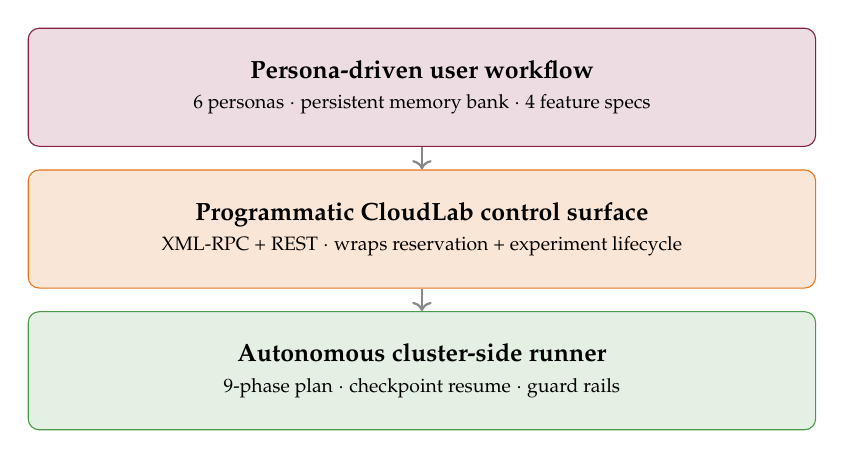
\begin{tikzpicture}[
  layer/.style={draw, rounded corners=4pt, minimum width=10cm,
                minimum height=1.5cm, align=center, font=\small},
]
  \node[layer, fill=myRed!15, draw=myRed] (l1) at (0,2.4) {
    \textbf{Persona-driven user workflow}\\
    {\scriptsize 6 personas $\cdot$ persistent memory bank $\cdot$ 4 feature specs}
  };
  \node[layer, fill=myOrange!18, draw=myOrange] (l2) at (0,0.6) {
    \textbf{Programmatic CloudLab control surface}\\
    {\scriptsize XML-RPC + REST $\cdot$ wraps reservation + experiment lifecycle}
  };
  \node[layer, fill=mGreen!15, draw=mGreen] (l3) at (0,-1.2) {
    \textbf{Autonomous cluster-side runner}\\
    {\scriptsize 9-phase plan $\cdot$ checkpoint resume $\cdot$ guard rails}
  };
  \draw[->, thick, mGray] (l1) -- (l2);
  \draw[->, thick, mGray] (l2) -- (l3);
\end{tikzpicture}
\note{
  \textbf{Key point:} Three coupled layers, each with named in-tree artifacts.\\
  \textbf{Say:} The project is more orchestration than research---five methods,
  two transports, sub-day reservation windows, six-day scheduler outage.
  We organized it as three coupled layers. Top: persona-driven user workflow.
  Six personas (feature-architect, construction-lead, knowledge-steward,
  memory-agent, etc.) with a persistent memory bank and four feature specs
  that survived three reality pivots. Middle: a programmatic CloudLab control
  surface wrapping the XML-RPC and web APIs. Bottom: an autonomous
  cluster-side runner that executed a 9-phase plan over 24 hours without
  a human in the chair.\\
  \textbf{Transition:} Two of these layers worked. The middle one half-worked,
  and that's where the story gets interesting.\\
  \textbf{Time:} 50s
}
\end{frame}

\begin{frame}{Layer 1: Persona-Driven User Workflow}
\centering
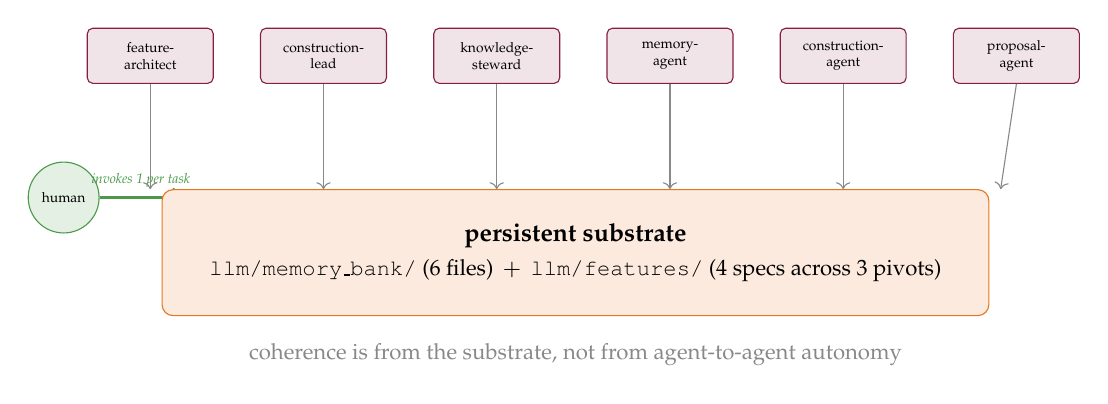
\begin{tikzpicture}[
  persona/.style={draw, rounded corners=2pt, minimum width=1.6cm,
                  minimum height=0.7cm, align=center, font=\tiny,
                  fill=myRed!12, draw=myRed},
  substrate/.style={draw, rounded corners=4pt, minimum width=10.5cm,
                    minimum height=1.6cm, align=center, font=\small,
                    fill=myOrange!15, draw=myOrange},
  human/.style={draw, circle, minimum size=0.9cm, align=center, font=\tiny,
                fill=mGreen!15, draw=mGreen},
]
  \node[persona] (p1) at (-5.4, 2.2) {feature-\\architect};
  \node[persona] (p2) at (-3.2, 2.2) {construction-\\lead};
  \node[persona] (p3) at (-1.0, 2.2) {knowledge-\\steward};
  \node[persona] (p4) at ( 1.2, 2.2) {memory-\\agent};
  \node[persona] (p5) at ( 3.4, 2.2) {construction-\\agent};
  \node[persona] (p6) at ( 5.6, 2.2) {proposal-\\agent};

  \node[human] (h) at (-6.5, 0.4) {human};
  \draw[->, thick, mGreen] (h.east) -- node[above, font=\tiny, mGreen]{\emph{invokes 1 per task}} (-5.0, 0.4);

  \node[substrate] (sub) at (0, -0.3) {
    \textbf{persistent substrate} \\[0.15em]
    {\footnotesize \texttt{llm/memory\_bank/} (6 files) $\,+\,$ \texttt{llm/features/} (4 specs across 3 pivots)}
  };

  \draw[->, mGray] (p1.south) -- ($(sub.north) + (-5.4, 0)$);
  \draw[->, mGray] (p2.south) -- ($(sub.north) + (-3.2, 0)$);
  \draw[->, mGray] (p3.south) -- ($(sub.north) + (-1.0, 0)$);
  \draw[->, mGray] (p4.south) -- ($(sub.north) + ( 1.2, 0)$);
  \draw[->, mGray] (p5.south) -- ($(sub.north) + ( 3.4, 0)$);
  \draw[->, mGray] (p6.south) -- ($(sub.north) + ( 5.4, 0)$);

  \node[font=\footnotesize, text=mGray] at (0, -1.6) {coherence is from the substrate, not from agent-to-agent autonomy};
\end{tikzpicture}
\note{
  \textbf{Key point:} Six personas, persistent substrate, human-invoked per task.\\
  \textbf{Say:} Six personas: feature-architect, construction-lead, knowledge-steward,
  memory-agent, construction-agent, proposal-agent. Each one invoked by the human
  per task --- not a self-orchestrating fleet. What made this work over six weeks
  is the substrate: a memory bank with six files read at the start of every session,
  and four feature specs authored when reality changed --- once in April when
  reservations failed and we pivoted to no-hardware, once in May when hardware
  finally worked and we reframed the contribution. The substrate held up; the
  personas don't auto-handoff. That's the methodology contribution.\\
  \textbf{Transition:} The middle layer is where the agent approach hits the wall.\\
  \textbf{Time:} 60s
}
\end{frame}

\begin{frame}{Layer 2: CloudLab Control Surface --- and Where It Breaks}
\centering
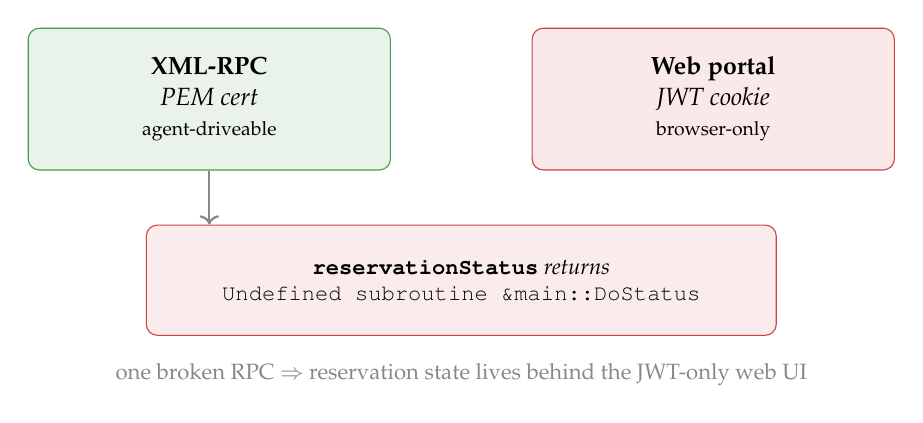
\begin{tikzpicture}[
  surface/.style={draw, rounded corners=4pt, minimum width=4.6cm,
                  minimum height=1.8cm, align=center, font=\small},
  bug/.style={draw, rounded corners=4pt, minimum width=8cm,
              minimum height=1.4cm, align=center, font=\footnotesize,
              fill=mRed!10, draw=mRed},
  xmark/.style={text=mRed, font=\Huge\bfseries},
]
  \node[surface, fill=mGreen!12, draw=mGreen] (xmlrpc) at (-3.2, 1.6) {
    \textbf{XML-RPC}\\
    \emph{PEM cert}\\
    {\scriptsize agent-driveable}};
  \node[surface, fill=mRed!12, draw=mRed]   (web)    at ( 3.2, 1.6) {
    \textbf{Web portal}\\
    \emph{JWT cookie}\\
    {\scriptsize browser-only}};
  \node[xmark] at (0, 1.6) {$\nleftrightarrow$};

  \node[bug] (rpc) at (0, -0.7) {
    \textbf{\texttt{reservationStatus}} \emph{returns}\\
    \texttt{Undefined subroutine \&main::DoStatus}};
  \draw[->, thick, mGray] (xmlrpc.south) -- (rpc.north -| xmlrpc.south);
  \node[font=\footnotesize, text=mGray] at (0, -1.9) {one broken RPC $\Rightarrow$ reservation state lives behind the JWT-only web UI};
\end{tikzpicture}
\note{
  \textbf{Key point:} Two control planes, the bridge is broken.\\
  \textbf{Say:} CloudLab has two control surfaces. The XML-RPC side accepts
  PEM client certs --- an agent can drive that. The web portal accepts JWT
  cookies --- an agent without a browser cannot. They don't interoperate:
  PEM against the web returns empty, JWT against XML-RPC returns 404. This
  was workable until \texttt{reservationStatus} returned a server-side Perl
  bug --- \texttt{Undefined subroutine \&main::DoStatus}. With that one RPC
  broken, the only path to inspect reservation state was the JWT-only web
  UI. That cost us six days.\\
  \textbf{Transition:} The bottom layer worked despite all this --- here's how.\\
  \textbf{Time:} 55s
}
\end{frame}

\begin{frame}{Layer 3: Autonomous Runner $+$ ORNL XLOOP'25 Differentiation}
\centering
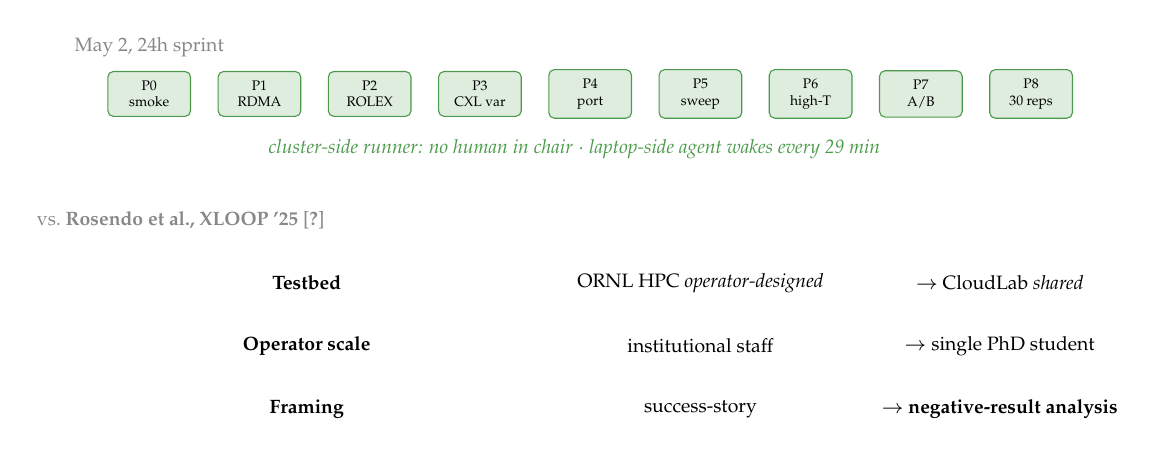
\begin{tikzpicture}[
  phase/.style={draw, rounded corners=2pt, minimum width=1.05cm,
                minimum height=0.55cm, align=center, font=\tiny,
                fill=mGreen!18, draw=mGreen},
  diffrow/.style={align=center, font=\scriptsize},
]
  % Top half: 24-hour sprint timeline
  \node[font=\scriptsize, text=mGray] at (-5.4, 2.6) {May 2, 24h sprint};
  \foreach \x/\lab in {-5.4/{P0\\smoke}, -4.0/{P1\\RDMA}, -2.6/{P2\\ROLEX}, -1.2/{P3\\CXL var}, 0.2/{P4\\port}, 1.6/{P5\\sweep}, 3.0/{P6\\high-T}, 4.4/{P7\\A/B}, 5.8/{P8\\30 reps}} {
    \node[phase] at (\x, 2.0) {\lab};
  }
  \node[font=\scriptsize, text=mGreen] at (0, 1.3) {\textit{cluster-side runner: no human in chair $\cdot$ laptop-side agent wakes every 29 min}};

  % Bottom half: ORNL XLOOP'25 differentiation 3-row table
  \node[font=\scriptsize, text=mGray] at (-5, 0.4) {vs.\ \textbf{Rosendo et al., XLOOP '25}~\cite{ornl-agents-xloop25}};
  \node[diffrow] at (-3.4, -0.4) {\textbf{Testbed}};
  \node[diffrow] at (1.6,  -0.4) {ORNL HPC \emph{operator-designed}};
  \node[diffrow] at (5.4,  -0.4) {$\rightarrow$ CloudLab \emph{shared}};
  \node[diffrow] at (-3.4, -1.2) {\textbf{Operator scale}};
  \node[diffrow] at (1.6,  -1.2) {institutional staff};
  \node[diffrow] at (5.4,  -1.2) {$\rightarrow$ single PhD student};
  \node[diffrow] at (-3.4, -2.0) {\textbf{Framing}};
  \node[diffrow] at (1.6,  -2.0) {success-story};
  \node[diffrow] at (5.4,  -2.0) {$\rightarrow$ \textbf{negative-result analysis}};
\end{tikzpicture}
\note{
  \textbf{Key point:} Bottom layer worked. Differentiation from ORNL preempts the obvious objection.\\
  \textbf{Say:} The bottom layer is the only one that ran without me in
  the chair. May 2 sprint, nine phases, twenty-four hours: cluster-side
  runner drove workloads, the resilient runner wrapped each one with
  checkpoint resume, two guard scripts caught control-net violations.
  Laptop-side agent woke every twenty-nine minutes --- under the prompt
  cache window --- pulled results via scp, plotted, committed. The closest
  published prior art is Rosendo et al., XLOOP '25, on AI agents for HPC
  user facilities at ORNL. Three differentiations: they target internal
  facilities with operator-designed infrastructure; we target a shared
  academic testbed where the gaps are the contribution. Institutional
  scale versus a single PhD student. Their paper is a success story;
  this is a negative-result analysis.\\
  \textbf{Transition:} Now the case study --- starting with what Sherman tells us.\\
  \textbf{Time:} 60s
}
\end{frame}


% ============================================================
% SECTION 4: Stress-Testing Finding (1 spoken slide)
% ============================================================

\section{Stress-Testing Finding}

\begin{frame}[fragile]{Sherman LOAD Crash on RDMA}
\centering
\begin{lstlisting}[basicstyle=\ttfamily\small,backgroundcolor=\color{mGray!10},frame=single]
Assertion `k >= fence_keys.lowest' failed
  at src/Tree.cpp:382
\end{lstlisting}
\medskip
\textit{\small CHIME's \texttt{SIBLING\_BASED\_VALIDATION} $+$ \texttt{VACANCY\_AWARE\_LOCK} close the window. CHIME completes LOAD on the same input.}
\note{
  \textbf{Key point:} A stress finding independent of the CXL story; empirical proof CHIME's techniques are jointly necessary for correctness.\\
  \textbf{Say:} While reproducing figure twelve, we tried Sherman LOAD at
  full per-CN concurrency. It crashed deterministically every time, around
  five million keys, on this assertion at Tree dot cpp line 382. The
  assertion has escape hatches for k greater than \emph{highest} (sibling walk),
  and for cache staleness, but no escape for k less than \emph{lowest} on a
  fresh non-cached read. Under concurrent borrow or merge that widens
  N's lower fence key before the parent pointer updates, a thread can
  descend through a stale parent into a node whose fence has just moved.
  CHIME's sibling-based validation and vacancy-aware lock close that
  window. CHIME completes LOAD on the same input; Sherman doesn't. So
  the crash is a baseline limitation, not a fixable bug --- it's empirical
  proof CHIME's techniques are jointly necessary for correctness, not
  just throughput.\\
  \textbf{Transition:} Now CXL --- where transport changes which features pay off.\\
  \textbf{Time:} 50s
}
\end{frame}


% ============================================================
% SECTION 5: CXL Findings (3 spoken slides)
% ============================================================

\section{CXL Findings}

\begin{frame}{CXL/RDMA Ratio: Workload-Dependent Win}
\centering
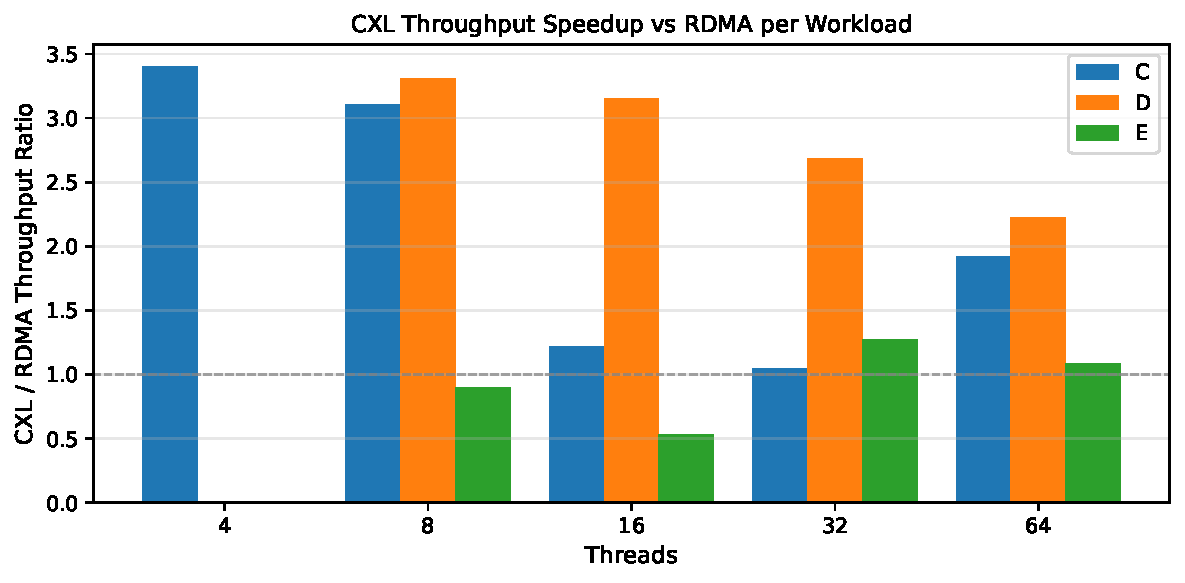
\includegraphics[height=0.78\textheight]{../report/figures/fig12-cxl-rdma-ratio.pdf}
\note{
  \textbf{Key point:} The ratio chart isolates the workload-dependent CXL story.\\
  \textbf{Say:} This is the speedup ratio. Bars above one mean CXL wins; below one means RDMA wins. Read-heavy workloads C and D are uniformly above one. Range-scan E dips to roughly half RDMA at 16 threads, then crosses over at 32. The implication for a CXL-native CHIME is concrete: a transport-only port leaves the range-scan optimization on the table. A CXL-native scan would need either prefetch hints or helper threads to recover the in-flight pipelining that RDMA gets from coroutines.\\
  \textbf{Transition:} The infrastructure side wasn't as fortunate.\\
  \textbf{Time:} 50s
}
\end{frame}

\begin{frame}{Cross-Day Reproducibility: CXL Stable, RDMA Bimodal}
\centering
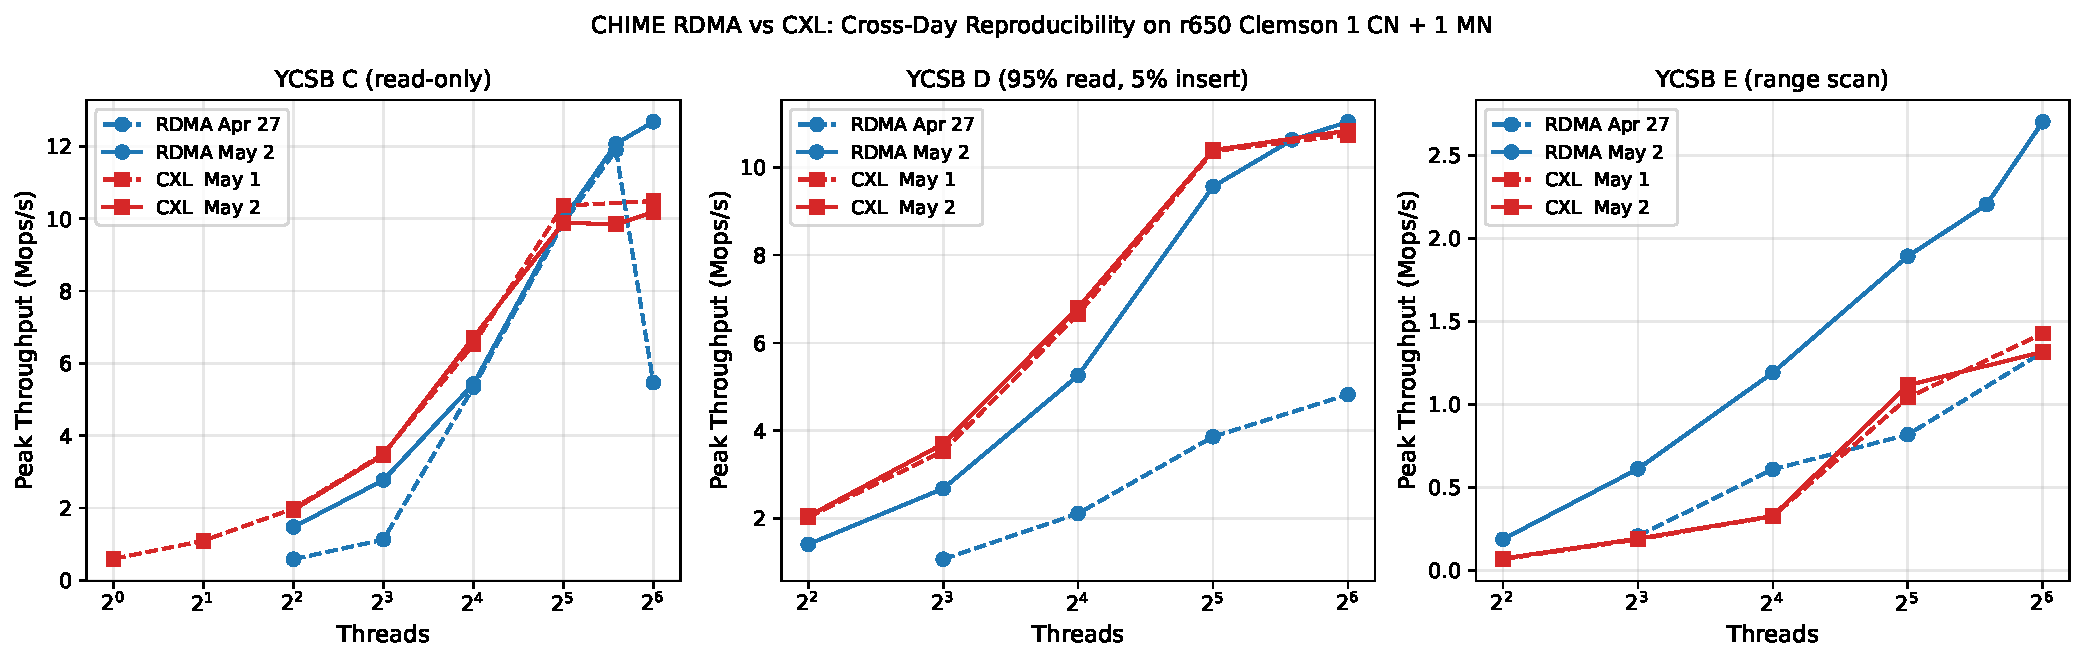
\includegraphics[height=0.65\textheight]{../report/figures/fig12-cxl-reproducibility.pdf}
\note{
  \textbf{Key point:} The cleanest reproducibility finding from the project: CHIME-CXL re-runs to within five percent across days; CHIME-RDMA varies by up to two-times.\\
  \textbf{Say:} Two re-runs on the same hardware. CHIME-CXL on May 1 versus May 2 reproduces within five percent on every workload. CHIME-RDMA on April 27 versus May 2 differs by up to two-times. The likely mechanism is the same warm-versus-cold cache bimodality we showed for the sixteen-thread variance reps. CXL has no such bimodality because there is no NIC-side queue to warm up. So the CXL/RDMA speedup ratio depends on which RDMA reference you use --- the April baseline gave a three-times speedup, the May baseline gives one-point-zero to one-point-four. Workload direction is robust; magnitude is reference-dependent. The reproducibility finding itself is the more interesting story: CXL is a more stable benchmark target than RDMA on shared cluster hardware.\\
  \textbf{Transition:} The infrastructure side wasn't as fortunate.\\
  \textbf{Time:} 50s
}
\end{frame}

% CUT-HERE-IF-SHORT  (slide 11 — drop cleanly if rehearsal > 13:00)
\begin{frame}{CXL fig\_15a: Speculative Read Can Hurt on CXL}
\centering
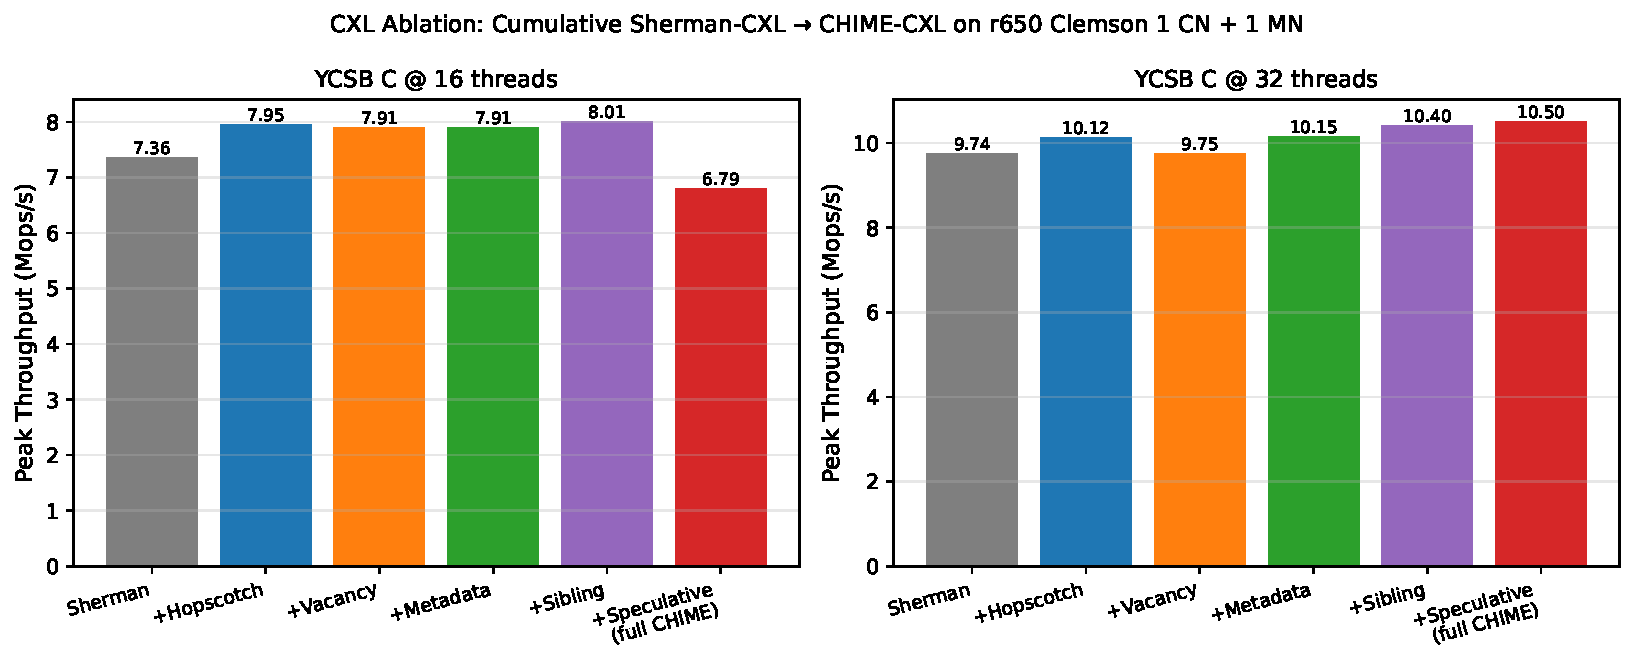
\includegraphics[height=0.65\textheight]{../report/figures/fig15a-cxl-ablation.pdf}
\note{
  \textbf{Key point:} The optimization stack that maximizes RDMA throughput is not transport-independent. Speculative read --- the last bar in CHIME's RDMA fig\_15a --- can be NEGATIVE-value on CXL.\\
  \textbf{Say:} CXL fig\_15a on workload C, 16 and 32 threads. Full CHIME-CXL --- the rightmost bar --- is SLOWER than +Sibling at 16 threads. About 6.79 versus 8.01 Mops per second. At 32 threads CHIME-CXL barely edges +Sibling. Compare to the paper's RDMA fig\_15a where speculative read consistently adds a small positive delta at every thread count. The mechanism that makes speculative read worthwhile on RDMA --- starting an extra read in parallel to hide the round-trip --- has no payoff on a synchronous CXL transport. The second read just serializes with the first. Implication: a CXL-native CHIME successor would gain more from DISABLING speculative read than from keeping it. The optimization stack is transport-specific.\\
  \textbf{Transition:} The reproducibility finding is the cleanest data point we have.\\
  \textbf{Time:} 45s
}
\end{frame}


% ============================================================
% SECTION 6: CloudLab Postmortem (2 spoken slides)
% ============================================================

\section{CloudLab Postmortem}

% Slide — The Misleading Error
\begin{frame}[fragile]{The Misleading Scheduler Error}
\begin{lstlisting}[basicstyle=\ttfamily\scriptsize,backgroundcolor=\color{mGray!10},frame=single,breaklines=true]
*** Resource reservation violation: 2 nodes of type
    r650 requested, but only 0 available because of
    existing resource reservations to other projects
    or users.
\end{lstlisting}
\centering\textit{\small ``Other projects or users'' --- but our reservations \emph{were} CS620426SP.}
\note{
  \textbf{Key point:} The error blames other projects, but the held capacity was OURS.\\
  \textbf{Say:} Every startExperiment over those six days returned within
  ninety seconds with this error. ``Other projects or users'' --- but I
  could see in the web UI that my own approved CS620426SP reservations
  were active. The capacity was ours; the scheduler just wasn't binding
  the experiment to it. To diagnose the mismatch, you'd run
  \texttt{reservationStatus}. That CLI returned a Perl runtime error
  --- \texttt{Undefined subroutine \&main::DoStatus} --- regardless of
  UUID. There is no client-side fix for that.\\
  \textbf{Transition:} Three concrete API additions would unblock this.\\
  \textbf{Time:} 55s
}
\end{frame}

% Slide — What Would Have Unblocked Us
\begin{frame}{Three CloudLab API Additions}
\centering
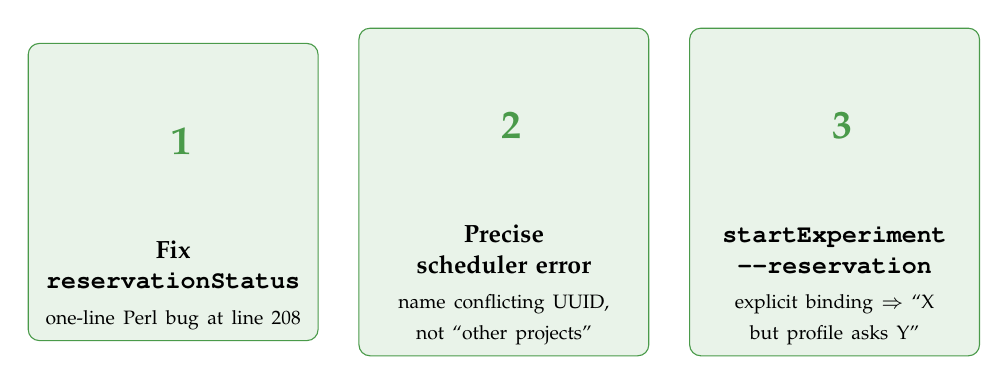
\begin{tikzpicture}[
  card/.style={draw, rounded corners=4pt, minimum width=3.6cm,
               minimum height=2.2cm, align=center, font=\small,
               text width=3.4cm, fill=mGreen!12, draw=mGreen,
               inner sep=4pt},
  num/.style={font=\Large\bfseries, text=mGreen},
]
  \node[card] (a) at (-4.2, 0) {
    \tikz\node[num]{1};\\
    \textbf{Fix\\\texttt{reservationStatus}}\\[0.2em]
    {\scriptsize one-line Perl bug at line 208}};
  \node[card] (b) at ( 0,   0) {
    \tikz\node[num]{2};\\
    \textbf{Precise\\scheduler error}\\[0.2em]
    {\scriptsize name conflicting UUID, not ``other projects''}};
  \node[card] (c) at ( 4.2, 0) {
    \tikz\node[num]{3};\\
    \textbf{\texttt{startExperiment\\-{}-reservation}}\\[0.2em]
    {\scriptsize explicit binding $\Rightarrow$ ``X but profile asks Y''}};
\end{tikzpicture}

\medskip
\centering\textit{\small each independently sufficient to surface root cause in the first failed window}
\note{
  \textbf{Key point:} Three engineering fixes, each independently sufficient.\\
  \textbf{Say:} Three concrete API improvements, each individually sufficient
  to have surfaced our root cause inside the first failed reservation window.
  One: fix the \texttt{reservationStatus} RPC --- it's a one-line Perl bug.
  Two: make the scheduler error name the conflicting reservation UUID,
  instead of saying ``other projects or users'' when the holder is in fact
  the same project under an unmatched binding. Three: add an explicit
  \texttt{--reservation} flag to \texttt{startExperiment}, so the scheduler
  can return ``your reservation has hardware type X but the profile asks
  for Y.'' These are not editorial complaints. They are testable engineering
  changes. They are the contribution this layer claims.\\
  \textbf{Transition:} Closing the loop --- what the orchestration got us.\\
  \textbf{Time:} 60s
}
\end{frame}


% ============================================================
% SECTION 7: Closing (2 spoken slides)
% ============================================================

\section{Closing}

\begin{frame}[fragile]{From Crash to Throughput in One Line}
\centering
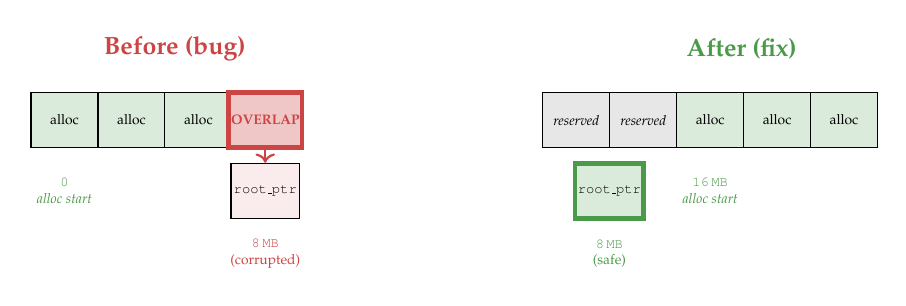
\begin{tikzpicture}[
  region/.style={draw, minimum height=0.7cm, minimum width=0.85cm,
                 align=center, font=\tiny, inner sep=1pt},
  rootlabel/.style={font=\tiny, text=mRed, align=center},
  alloclabel/.style={font=\tiny, text=mGreen, align=center},
]
  % BEFORE
  \node[font=\small\bfseries, text=mRed] at (-3.6, 2.4) {Before (bug)};
  \node[region, fill=mGreen!20] (a0) at (-5.0, 1.5) {alloc};
  \node[region, fill=mGreen!20] at (-4.15, 1.5) {alloc};
  \node[region, fill=mGreen!20] at (-3.30, 1.5) {alloc};
  \node[region, fill=mRed!30, draw=mRed, ultra thick] (overlap1) at (-2.45, 1.5) {\bfseries\color{mRed}OVERLAP};
  \node[region, fill=mRed!10] (rp1) at (-2.45, 0.6) {\texttt{root\_ptr}};
  \node[rootlabel] at (-2.45, -0.2) {\texttt{8\,MB}\\(corrupted)};
  \node[alloclabel] at (-5.0, 0.6) {\texttt{0}\\\textit{alloc start}};
  \draw[->, thick, mRed] (overlap1.south) -- (rp1.north);

  % AFTER
  \node[font=\small\bfseries, text=mGreen] at (3.6, 2.4) {After (fix)};
  \node[region, fill=mGray!20] (res) at (1.5, 1.5) {\textit{reserved}};
  \node[region, fill=mGray!20] at (2.35, 1.5) {\textit{reserved}};
  \node[region, fill=mGreen!20] at (3.20, 1.5) {alloc};
  \node[region, fill=mGreen!20] at (4.05, 1.5) {alloc};
  \node[region, fill=mGreen!20] at (4.90, 1.5) {alloc};
  \node[region, fill=mGreen!20, draw=mGreen, ultra thick] (rp2) at (1.92, 0.6) {\texttt{root\_ptr}};
  \node[rootlabel, text=mGreen] at (1.92, -0.2) {\texttt{8\,MB}\\(safe)};
  \node[alloclabel] at (3.20, 0.6) {\texttt{16\,MB}\\\textit{alloc start}};
\end{tikzpicture}

\medskip\centering\small
\texttt{alloc\_offset\_(define::kChunkSize)}\quad{\color{mGreen}\textbf{commit \texttt{a3c9e87}}}
\quad$\to$\quad\textbf{0.6\,Mops/s, 10 epochs, no segfault}
\note{
  \textbf{Key point:} The CXL bug was a one-line allocator overlap. The fix was found because the orchestration captured the trace.\\
  \textbf{Say:} Closing the loop on the orchestration claim. Three reservations
  crashed before this got fixed. The fix turned out to be one line: the
  CXL allocator started at offset zero, growing linearly; the tree's root
  pointer lives at offset eight megabytes. Once allocations crossed eight
  megabytes, alloc handed back addresses on top of the root pointer,
  corrupting it. The instrumented trace --- written by the cluster-side
  runner into NFS --- showed the level-four root pointer flip to a
  level-thirty-three-thousand garbage value, then segfault. The fix is
  to start the allocator at sixteen megabytes. One line, commit a3c9e87.
  YCSB-C ran clean to ten epochs at 0.6 megaops per second. The bug is
  found because the orchestration captured the failure --- not because
  I was at the keyboard during the crash.\\
  \textbf{Transition:} Three takeaways.\\
  \textbf{Time:} 50s
}
\end{frame}

% Slide 25 — Key Takeaways (rewritten by reframe spec to lead with orchestration)
\begin{frame}{Key Takeaways}
\centering
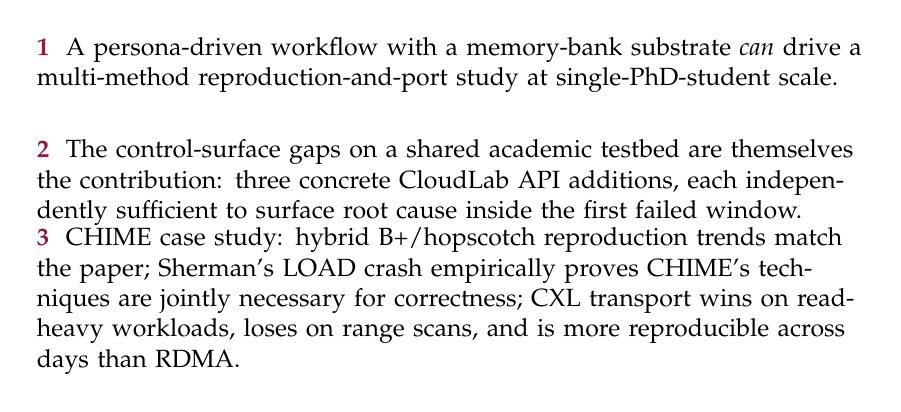
\begin{tikzpicture}[
  item/.style={font=\small, anchor=west, text width=10.5cm},
]
  \node[item] at (-5.3, 2.2)   {{\color{myRed}\textbf{1}}~~A persona-driven workflow with a memory-bank substrate \emph{can} drive a multi-method reproduction-and-port study at single-PhD-student scale.};
  \node[item] at (-5.3, 0.7)   {{\color{myRed}\textbf{2}}~~The control-surface gaps on a shared academic testbed are themselves the contribution: three concrete CloudLab API additions, each independently sufficient to surface root cause inside the first failed window.};
  \node[item] at (-5.3,-0.8)   {{\color{myRed}\textbf{3}}~~CHIME case study: hybrid B+/hopscotch reproduction trends match the paper; Sherman's LOAD crash empirically proves CHIME's techniques are jointly necessary for correctness; CXL transport wins on read-heavy workloads, loses on range scans, and is more reproducible across days than RDMA.};
\end{tikzpicture}
\note{
  \textbf{Key point:} Three closing points, leading with orchestration.\\
  \textbf{Say:} Three takeaways. First, a persona-driven workflow with a
  memory-bank substrate---not a self-orchestrating fleet, but a substrate
  that survives session boundaries---can drive a multi-method
  reproduction-and-port study at single-PhD-student scale. Second, the
  control-surface gaps on a shared academic testbed like CloudLab are
  themselves the contribution: three concrete API additions inferred from
  where the agent approach broke, each individually sufficient to surface
  root cause inside the first failed reservation window. Third, on the
  CHIME case study itself: hybrid B+/hopscotch reproduction trends match
  the paper; Sherman's LOAD crash empirically proves CHIME's techniques
  are jointly necessary for correctness, not just throughput; and CXL
  transport wins on read-heavy workloads, loses on range scans, and is
  more reproducible across days than RDMA. That's the project.\\
  \textbf{Transition:} Thank you.\\
  \textbf{Time:} 50s
}
\end{frame}


% ============================================================
% APPENDIX BEGINS — frames after this are backup / Q&A material
% Suppress the section-navigation headline for appendix slides so the
% nav bar doesn't overflow with backup section names.
% ============================================================

\appendix
\setbeamertemplate{headline}{}

\section{Backup: Paper Overview}

% Slide 2 — The Problem
\begin{frame}{Disaggregated Memory Indexes}
\centering
\includegraphics[height=0.82\textheight]{diagrams/tradeoff.pdf}
\note{
  \textbf{Key point:} DM range indexes face a cache vs read-amp trade-off.\\
  \textbf{Say:} Disaggregated memory separates compute and memory over
  a network. Range indexes on DM face a fundamental trade-off: B+ trees
  cache well but need multiple round trips per lookup, while hash indexes
  are fast but consume huge cache. CHIME breaks this trade-off.\\
  \textbf{Transition:} Here's how CHIME does it.\\
  \textbf{Time:} 45s
}
\end{frame}

% Slide 3 — The Insight
\begin{frame}{CHIME: Hybrid Structure}
\centering
\includegraphics[height=0.82\textheight]{diagrams/hybrid-structure.pdf}
\note{
  \textbf{Key point:} Hybrid = tree structure + hash leaves.\\
  \textbf{Say:} CHIME keeps B+ tree internal nodes for structure
  and range query support, but replaces sorted leaves with
  hopscotch hashing. Internal nodes cache well because there
  are few of them. Leaves use hashing to find keys in one
  round trip instead of binary search.\\
  \textbf{Transition:} Three specific techniques make this work.\\
  \textbf{Time:} 45s
}
\end{frame}

% Slide 4 — Three Techniques
\begin{frame}{Three Key Techniques}
\centering
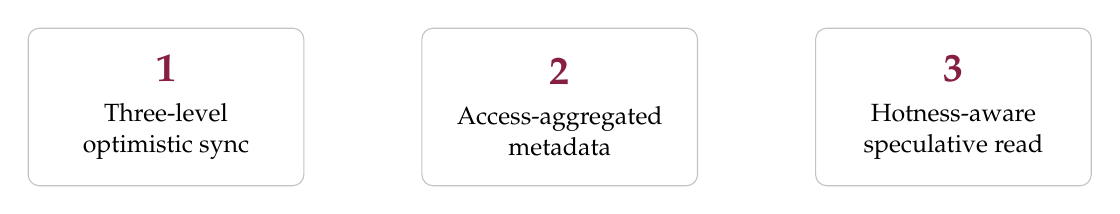
\begin{tikzpicture}[
  card/.style={draw=mGray!50, rounded corners=4pt, minimum width=3.5cm,
               minimum height=2cm, align=center, font=\small},
]
  \node[card] (t1) at (-5,0) {
    {\Large\color{mTeal} \textbf{1}}\\[0.4em]
    Three-level\\optimistic sync
  };
  \node[card] (t2) at (0,0) {
    {\Large\color{mTeal} \textbf{2}}\\[0.4em]
    Access-aggregated\\metadata
  };
  \node[card] (t3) at (5,0) {
    {\Large\color{mTeal} \textbf{3}}\\[0.4em]
    Hotness-aware\\speculative read
  };
\end{tikzpicture}
\note{
  \textbf{Key point:} Three techniques enable the hybrid design.\\
  \textbf{Say:} Three techniques make this work. First, three-level
  optimistic synchronization reuses hopscotch bitmaps for fine-grained
  concurrency---no global locks. Second, vacancy bitmap piggybacking
  and metadata replication reduce round trips for metadata. Third,
  a hotspot buffer shortcuts reads for frequently accessed neighborhoods.\\
  \textbf{Transition:} What does this achieve?\\
  \textbf{Time:} 50s
}
\end{frame}

% Slide — CHIME's Five Techniques (detailed)
\begin{frame}{CHIME's Five Techniques (CMake Flags)}
\small Each technique adds an RDMA-amortizing optimization on top of a hopscotch-leaf B+~tree:
\vspace{0.3em}
\begin{center}
\begin{tabular}{@{}lp{8.2cm}@{}}
\toprule
\textbf{CMake Flag} & \textbf{What It Does} \\
\midrule
\texttt{HOPSCOTCH\_LEAF\_NODE} & Hash-based leaf nodes; finds key in 1 RTT instead of binary-search \\
\texttt{VACANCY\_AWARE\_LOCK}  & Lock word piggybacks vacancy bitmap; insert sees lock + free slot in one read \\
\texttt{METADATA\_REPLICATION} & Per-segment replicated metadata; saves 1 RTT per leaf access \\
\texttt{SIBLING\_BASED\_VALIDATION} & Sibling fence-key check on every read; catches stale-cache without re-read \\
\texttt{SPECULATIVE\_READ}     & Hotspot buffer; warm keys shortcut neighborhood scan \\
\bottomrule
\end{tabular}
\end{center}
\vspace{0.5em}
{\small The paper's fig\_15a evaluates these by toggling them \emph{cumulatively} on top of a Sherman baseline.}
\note{
  \textbf{Key point:} The 5 specific features that the paper ablates.\\
  \textbf{Say:} The paper isolates five techniques. Hopscotch leaves are the
  structural change — hash-based leaves replace sorted B+ leaves. The other
  four are RDMA optimizations: vacancy-aware lock piggybacks the vacancy
  bitmap on the lock word so an insert's lock-acquisition read also tells
  it which slot is free. Metadata replication trades a small per-segment
  size for a saved RTT on every leaf access. Sibling-based validation
  catches stale caches via cross-validation against the sibling pointer's
  fence keys. Speculative read shortcuts the neighborhood scan for hot
  keys. We'll see fig\_15a reproduce these later.\\
  \textbf{Transition:} Here's CHIME's headline claim.\\
  \textbf{Time:} 75s
}
\end{frame}

% Slide — Paper's Published Results
\begin{frame}{Paper's Published Throughput-Latency Curves}
\centering
\IfFileExists{../report/figures/fig12-paper.png}{%
  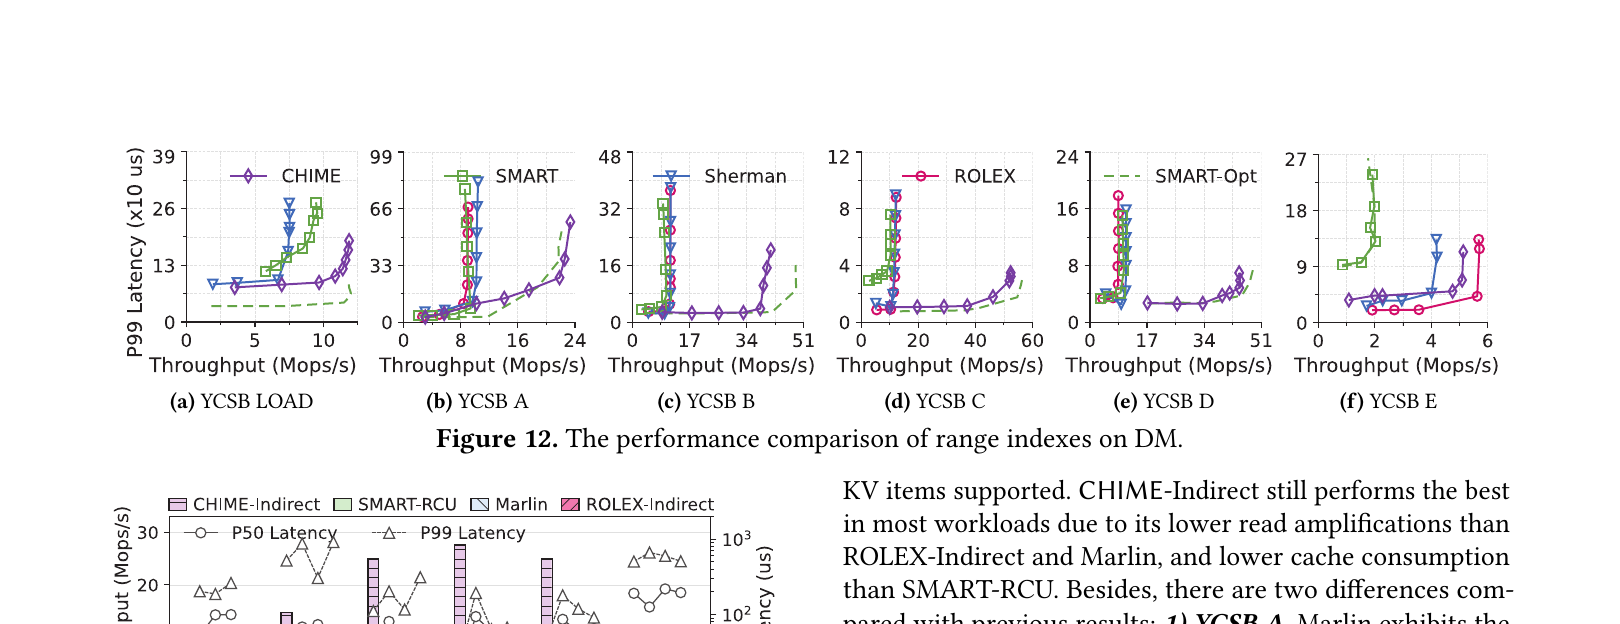
\includegraphics[width=0.95\textwidth]{../report/figures/fig12-paper.png}%
}{%
  \begin{tikzpicture}
    \draw[mGray!40, dashed, rounded corners=4pt] (0,0) rectangle (10,5);
    \node[mGray] at (5,2.5) {[fig\_12 from Bang et al.\ SOSP '24]};
  \end{tikzpicture}%
}
\vspace{0.3em}

{\scriptsize Source: Bang et al., \emph{CHIME: A Cache-Efficient and High-Performance Hybrid Index on Disaggregated Memory}, SOSP '24, Figure 12 (LOAD/A/B/C/D/E across CHIME, SMART, Sherman, ROLEX, SMART-Opt).}
\note{
  \textbf{Key point:} The paper's headline result we are trying to reproduce.\\
  \textbf{Say:} This is fig 12 from the paper. Throughput on the x-axis,
  P99 latency on the y-axis. Each panel is a YCSB workload — LOAD, A, B,
  C, D, E. Six panels, five methods per panel. CHIME's curves push to the
  right (higher throughput) and stay low (lower latency) compared to the
  baselines. The paper reports 2 to 5.6 times higher peak throughput than
  the next-best baseline on read-heavy workloads. Our job is to reproduce
  the trends on CloudLab r650 hardware.\\
  \textbf{Transition:} The headline claim.\\
  \textbf{Time:} 60s
}
\end{frame}

% Slide 5 — The Claim
{
\setbeamercolor{background canvas}{bg=myRed}
\begin{frame}[plain]
\vspace*{\fill}
\begin{center}
{\color{white}\Huge\bfseries 2.0--5.6\texttimes{} throughput}
\end{center}
\vspace*{\fill}
\note{
  \textbf{Key point:} CHIME's headline result.\\
  \textbf{Say:} The paper claims CHIME achieves 2.0 to 5.6 times higher
  throughput than state-of-the-art DM indexes while using comparable
  or less cache. Our job: reproduce this on real hardware.\\
  \textbf{Transition:} Let me describe our experimental setup.\\
  \textbf{Time:} 20s
}
\end{frame}
}

\section{Backup: Setup Detail}

% Slide 8 — What We Measured
\begin{frame}{What We Measured}
\centering
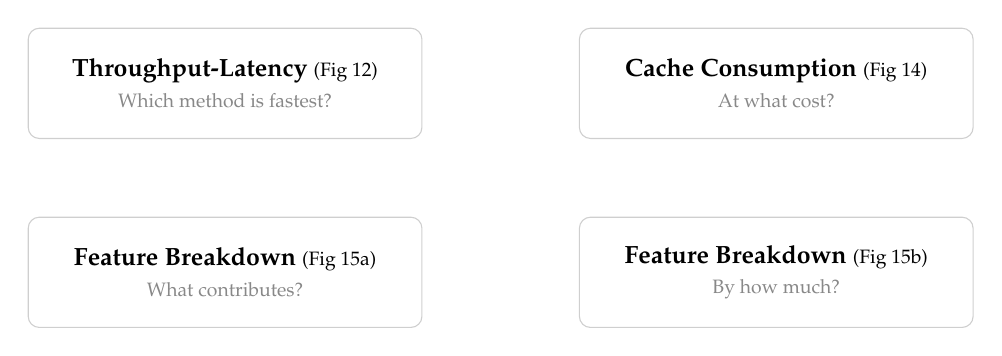
\begin{tikzpicture}[
  card/.style={draw=mGray!40, rounded corners=4pt, minimum width=5cm,
               minimum height=1.4cm, align=center, font=\small},
]
  \node[card] at (-3.5,1.2) {
    \textbf{Throughput-Latency} {\scriptsize(Fig~12)}\\
    {\color{mGray}\scriptsize Which method is fastest?}
  };
  \node[card] at (3.5,1.2) {
    \textbf{Cache Consumption} {\scriptsize(Fig~14)}\\
    {\color{mGray}\scriptsize At what cost?}
  };
  \node[card] at (-3.5,-1.2) {
    \textbf{Feature Breakdown} {\scriptsize(Fig~15a)}\\
    {\color{mGray}\scriptsize What contributes?}
  };
  \node[card] at (3.5,-1.2) {
    \textbf{Feature Breakdown} {\scriptsize(Fig~15b)}\\
    {\color{mGray}\scriptsize By how much?}
  };
\end{tikzpicture}
\note{
  \textbf{Key point:} Four core experiments targeting different aspects.\\
  \textbf{Say:} Four core experiments. Figure 12 is the main comparison---
  throughput vs latency across YCSB workloads. Figure 14 shows how much
  cache each method consumes. Figures 15a and 15b break down which CHIME
  techniques contribute how much performance.\\
  \textbf{Transition:} Here's our timeline for running these.\\
  \textbf{Time:} 45s
}
\end{frame}

% Slide 9 — Timeline
\begin{frame}{Experiment Timeline}
\centering
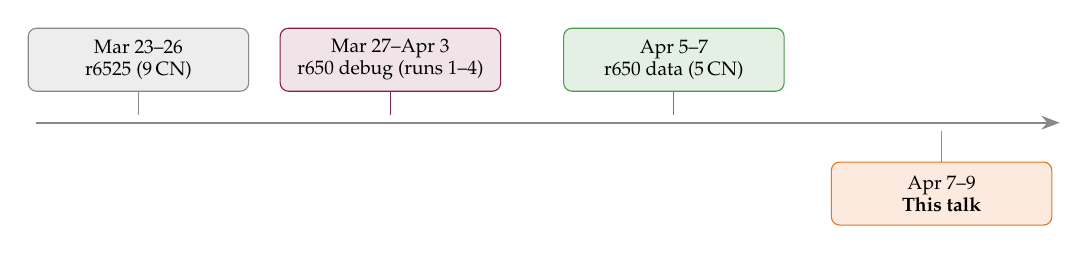
\begin{tikzpicture}[
  >=Stealth,
  milestone/.style={draw, rounded corners=3pt, minimum height=0.8cm,
                    align=center, font=\scriptsize, minimum width=2.8cm},
]
  % Timeline arrow
  \draw[->, thick, mGray] (-6.5,0) -- (6.5,0);

  % Milestones
  \node[milestone, fill=mGray!15, draw=mGray] at (-5.2,0.8) {
    Mar 23--26\\r6525 (9\,CN)
  };
  \draw[mGray] (-5.2,0.4) -- (-5.2,0.1);

  \node[milestone, fill=mTeal!12, draw=mTeal] at (-2,0.8) {
    Mar 27--Apr 3\\r650 debug (runs 1--4)
  };
  \draw[mTeal] (-2,0.4) -- (-2,0.1);

  \node[milestone, fill=mGreen!15, draw=mGreen] at (1.6,0.8) {
    Apr 5--7\\r650 data (5\,CN)
  };
  \draw[mGreen] (1.6,0.4) -- (1.6,0.1);

  \node[milestone, fill=mBrown!15, draw=mBrown] at (5,-0.9) {
    Apr 7--9\\\textbf{This talk}
  };
  \draw[mBrown] (5,-0.5) -- (5,-0.1);
\end{tikzpicture}
\note{
  \textbf{Key point:} Four phases of experiment runs.\\
  \textbf{Say:} Our timeline. Pre-deadline we ran on r6525---AMD, different
  from the paper's Intel. Then four runs on r650 debugging RDMA over RoCE---
  turns out you need an internal VLAN, not the control network. Finally
  this weekend we collected hardware-matched data on 5 compute nodes.\\
  \textbf{Transition:} Let me tell you what happened.\\
  \textbf{Time:} 30s
}
\end{frame}

\section{Backup: Reproduction Experience}

% Slide 10 — Challenge: Hardware Mismatch
\begin{frame}{Challenge: Hardware Mismatch}
\centering
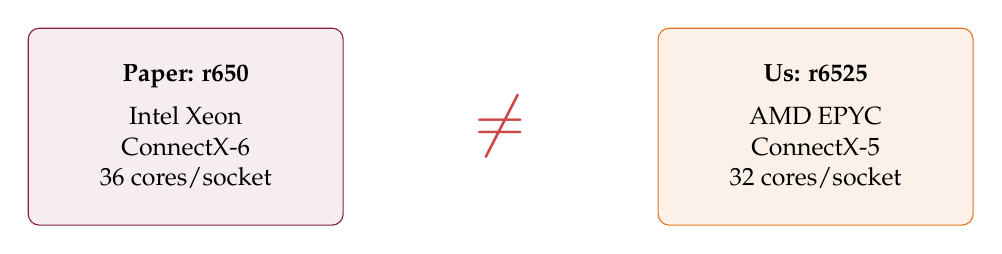
\begin{tikzpicture}[
  box/.style={draw, rounded corners=4pt, minimum width=4cm,
              minimum height=2.5cm, align=center, font=\small},
]
  \node[box, draw=mTeal, fill=mTeal!8] (paper) at (-4,0) {
    \textbf{Paper: r650}\\[0.5em]
    Intel Xeon\\
    ConnectX-6\\
    36 cores/socket
  };
  \node[box, draw=mBrown, fill=mBrown!10] (ours) at (4,0) {
    \textbf{Us: r6525}\\[0.5em]
    AMD EPYC\\
    ConnectX-5\\
    32 cores/socket
  };
  \node[font=\Huge, mRed] at (0,0) {$\neq$};
\end{tikzpicture}
\note{
  \textbf{Key point:} We had to use different hardware than the paper.\\
  \textbf{Say:} Our first challenge: r650 nodes were fully booked until
  after the deadline. We pivoted to r6525 nodes---AMD instead of Intel,
  different NIC. We had to validate that RDMA features like DCT actually
  worked on this hardware. They did, but we can't directly compare our
  numbers to the paper's.\\
  \textbf{Transition:} That wasn't the only problem.\\
  \textbf{Time:} 50s
}
\end{frame}

% Slide 11 — Challenge: Broken Node
\begin{frame}{Challenge: Broken Node}
\centering
\includegraphics[height=0.82\textheight]{diagrams/broken-node.pdf}
\note{
  \textbf{Key point:} Lost a node to hardware failure.\\
  \textbf{Say:} Node 10 had a broken RDMA interface. We couldn't replace
  it---CloudLab reservations are fixed. So we ran with 9 compute nodes
  instead of 10. This matches our upcoming r650 run but means figure 12's
  CN scaling won't match the paper exactly.\\
  \textbf{Transition:} There were software issues too.\\
  \textbf{Time:} 45s
}
\end{frame}

% Slide 12 — Challenge: RoCE Configuration
\begin{frame}{Challenge: RDMA on Ethernet (RoCE)}
\centering
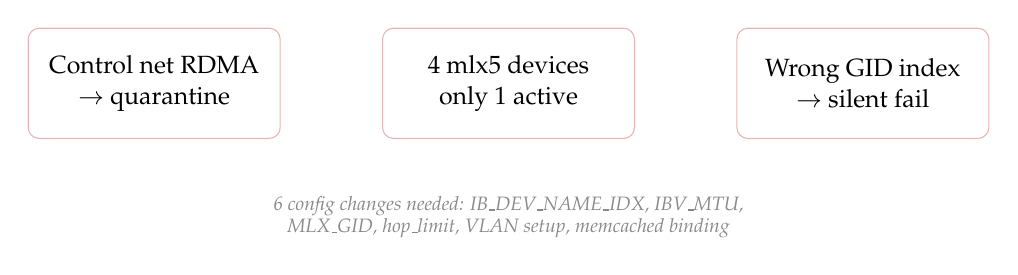
\begin{tikzpicture}[
  issue/.style={draw=mRed!40, rounded corners=4pt, minimum width=3.2cm,
                minimum height=1.4cm, align=center, font=\small},
]
  \node[issue] at (-4.5,0.5) {Control net RDMA\\$\to$ quarantine};
  \node[issue] at (0,0.5) {4 mlx5 devices\\only 1 active};
  \node[issue] at (4.5,0.5) {Wrong GID index\\$\to$ silent fail};
  \node[font=\scriptsize\itshape, mGray, align=center] at (0,-1.2)
    {6 config changes needed: IB\_DEV\_NAME\_IDX, IBV\_MTU,\\
     MLX\_GID, hop\_limit, VLAN setup, memcached binding};
\end{tikzpicture}
\note{
  \textbf{Key point:} r650 uses RoCE, not InfiniBand---6 config changes needed.\\
  \textbf{Say:} The hardest part: the r650 at Clemson uses RoCE---RDMA over
  Ethernet---not InfiniBand like the paper assumes. If you run RDMA on the
  control network, CloudLab quarantines your account. The NIC exposes 4
  mlx5 devices but only one is active. We needed to find the right device
  index, GID index, MTU, hop limit, and VLAN interface. This took four
  runs to debug---six separate config changes in total.\\
  \textbf{Transition:} There were other issues too.\\
  \textbf{Time:} 50s
}
\end{frame}

% Slide 13 — Challenge: Tooling Issues
\begin{frame}{Challenge: Tooling Issues}
\centering
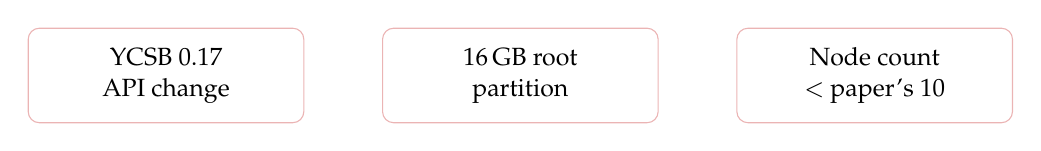
\begin{tikzpicture}[
  issue/.style={draw=mRed!40, rounded corners=4pt, minimum width=3.5cm,
                minimum height=1.2cm, align=center, font=\small},
]
  \node[issue] at (-4.5,0) {YCSB 0.17\\API change};
  \node[issue] at (0,0) {16\,GB root\\partition};
  \node[issue] at (4.5,0) {Node count\\$<$ paper's 10};
\end{tikzpicture}
\note{
  \textbf{Key point:} Three more tooling/environment issues.\\
  \textbf{Say:} Three more issues. YCSB changed its Java package name
  between versions---broke the workload generator. The r6525 root
  partition is only 16 gigs---builds and logs fill it fast, so we moved
  everything to NVMe. And we never got the paper's 10 compute nodes---
  r650 availability at Clemson is heavily contended.\\
  \textbf{Transition:} Here's what we did about each.\\
  \textbf{Time:} 50s
}
\end{frame}

% Slide 13 — What We Tried
\begin{frame}{Solutions}
\centering
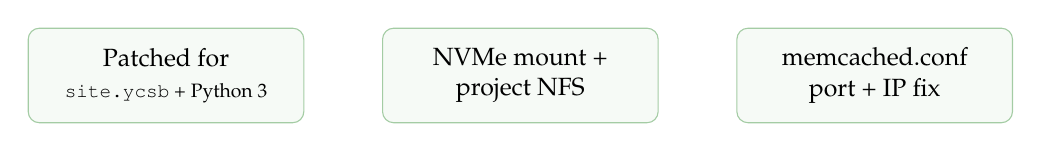
\begin{tikzpicture}[
  fix/.style={draw=mGreen!50, fill=mGreen!5, rounded corners=4pt,
              minimum width=3.5cm, minimum height=1.2cm,
              align=center, font=\small},
]
  \node[fix] at (-4.5,0) {Patched for\\{\scriptsize\texttt{site.ycsb} + Python~3}};
  \node[fix] at (0,0) {NVMe mount +\\project NFS};
  \node[fix] at (4.5,0) {memcached.conf\\port + IP fix};
\end{tikzpicture}
\note{
  \textbf{Key point:} Pragmatic fixes for each issue.\\
  \textbf{Say:} For each issue, we found pragmatic fixes. Patched the YCSB
  generator for the new API. Mounted NVMe drives and stored workloads on
  CloudLab's project NFS---which persists across experiments, so we only
  generate workloads once. And rewrote the memcached config for public IPs.\\
  \textbf{Transition:} The NFS solution was actually the biggest win.\\
  \textbf{Time:} 45s
}
\end{frame}

% Slide 14 — Key Win: Persistent Workloads
\begin{frame}{Key Win: Persistent Workloads}
\centering
\includegraphics[height=0.82\textheight]{diagrams/nfs-reuse.pdf}
\note{
  \textbf{Key point:} NFS persistence saved hours across runs.\\
  \textbf{Say:} The biggest win was persisting YCSB workloads on project
  NFS. Workload generation takes 90 minutes and produces gigabytes of data.
  By storing them on shared NFS, every experiment instance---r6525, r650,
  re-runs---just symlinks to the same data. Saved hours across our three
  reservation windows.\\
  \textbf{Transition:} Where do we stand now?\\
  \textbf{Time:} 40s
}
\end{frame}

% Slide 15 — Experiment Status
\begin{frame}{Experiment Status}
\centering
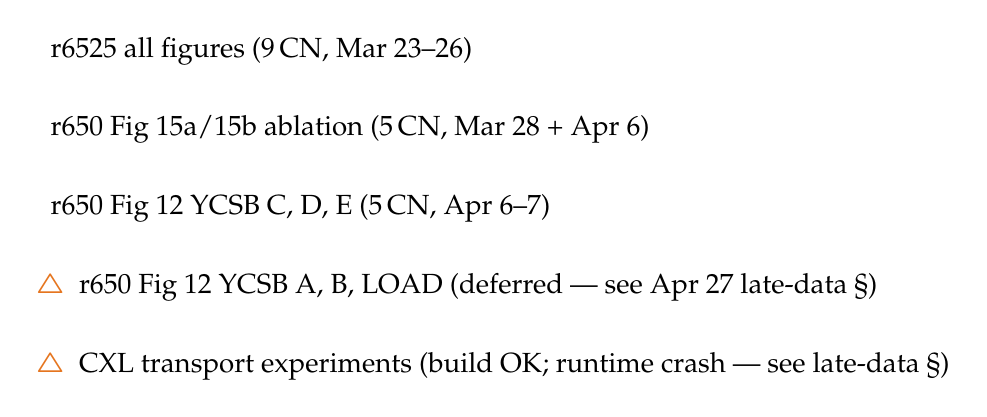
\begin{tikzpicture}[
  item/.style={font=\normalsize, anchor=west},
]
  \node[item] at (0, 2.0) {{\color{mGreen}\checkmark}~~r6525 all figures (9\,CN, Mar 23--26)};
  \node[item] at (0, 1.0) {{\color{mGreen}\checkmark}~~r650 Fig~15a/15b ablation (5\,CN, Mar 28 + Apr 6)};
  \node[item] at (0, 0.0) {{\color{mGreen}\checkmark}~~r650 Fig~12 YCSB C, D, E (5\,CN, Apr 6--7)};
  \node[item] at (0,-1.0) {{\color{mBrown}$\boldsymbol{\triangle}$}~~r650 Fig~12 YCSB A, B, LOAD (deferred --- see Apr~27 late-data \S)};
  \node[item] at (0,-2.0) {{\color{mBrown}$\boldsymbol{\triangle}$}~~CXL transport experiments (build OK; runtime crash --- see late-data \S)};
\end{tikzpicture}
\note{
  \textbf{Key point:} Most experiments complete on hardware-matched r650.\\
  \textbf{Say:} Status check. We completed all figures on r6525 pre-deadline,
  then re-ran on the paper-matched r650 hardware. Both ablation figures are
  complete. Fig~12 has three of six workloads done on r650, with the remaining
  three in progress. CXL experiments are planned for Part Two.\\
  \textbf{Transition:} What have we learned so far?\\
  \textbf{Time:} 30s
}
\end{frame}

% Slide 16 — Lessons So Far
\begin{frame}{Lessons Learned}
\centering
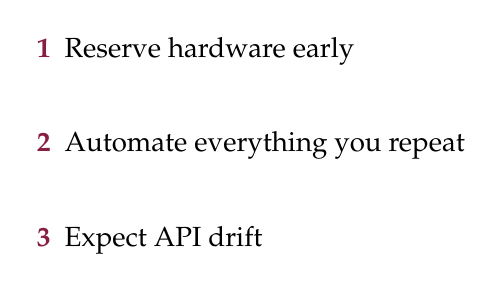
\begin{tikzpicture}[
  lesson/.style={font=\normalsize, anchor=west},
]
  \node[lesson] at (-3, 1.2) {{\color{mTeal}\textbf{1}}~~Reserve hardware early};
  \node[lesson] at (-3, 0)   {{\color{mTeal}\textbf{2}}~~Automate everything you repeat};
  \node[lesson] at (-3,-1.2) {{\color{mTeal}\textbf{3}}~~Expect API drift};
\end{tikzpicture}
\note{
  \textbf{Key point:} Three reproduction lessons.\\
  \textbf{Say:} Three lessons from reproduction. First, reserve CloudLab
  hardware weeks in advance---popular nodes book up fast. Second, automate
  setup scripts aggressively because you'll re-run them across multiple
  reservations. Third, don't assume open-source tooling is frozen---YCSB
  changed its API between releases and it broke our pipeline.\\
  \textbf{Transition:} Now let's look at what we expect from the experiments.\\
  \textbf{Time:} 45s
}
\end{frame}

\section{Backup: Methodology and Expected Results}

% Slide 17 — What We're Measuring
\begin{frame}{Methodology}
\centering
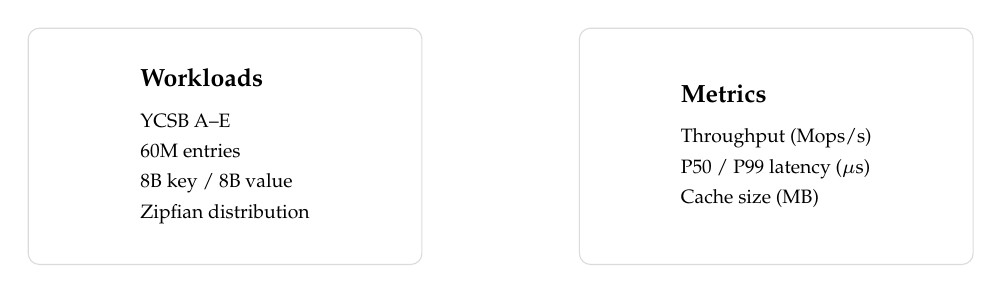
\begin{tikzpicture}[
  col/.style={draw=mGray!30, rounded corners=4pt, minimum width=5cm,
              minimum height=3cm, align=left, font=\small, anchor=north},
]
  \node[col] (wl) at (-3.5,1.5) {
    \textbf{Workloads}\\[0.4em]
    {\scriptsize YCSB A--E}\\
    {\scriptsize 60M entries}\\
    {\scriptsize 8B key / 8B value}\\
    {\scriptsize Zipfian distribution}
  };
  \node[col] (met) at (3.5,1.5) {
    \textbf{Metrics}\\[0.4em]
    {\scriptsize Throughput (Mops/s)}\\
    {\scriptsize P50 / P99 latency ($\mu$s)}\\
    {\scriptsize Cache size (MB)}
  };
\end{tikzpicture}
\note{
  \textbf{Key point:} Standard YCSB workloads with three metric dimensions.\\
  \textbf{Say:} Here's what we're running. YCSB workloads A through E---
  60 million entries, 8 byte keys and values, Zipfian distribution. We
  measure throughput in millions of operations per second, median and tail
  latency in microseconds, and cache consumption in megabytes.\\
  \textbf{Transition:} Based on the paper, here's what we expect.\\
  \textbf{Time:} 40s
}
\end{frame}

% Slide 18 — What We Expect
\begin{frame}{Expected Outcomes}
\centering
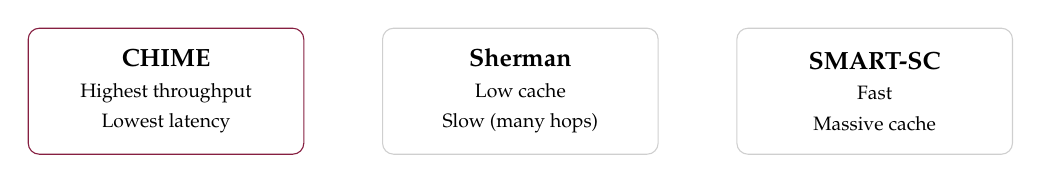
\begin{tikzpicture}[
  card/.style={draw=mGray!40, rounded corners=4pt, minimum width=3.5cm,
               minimum height=1.6cm, align=center, font=\small},
]
  \node[card, draw=mTeal] at (-4.5,0) {
    \textbf{CHIME}\\
    {\scriptsize Highest throughput}\\
    {\scriptsize Lowest latency}
  };
  \node[card] at (0,0) {
    \textbf{Sherman}\\
    {\scriptsize Low cache}\\
    {\scriptsize Slow (many hops)}
  };
  \node[card] at (4.5,0) {
    \textbf{SMART-SC}\\
    {\scriptsize Fast}\\
    {\scriptsize Massive cache}
  };
\end{tikzpicture}
\note{
  \textbf{Key point:} Predictions based on the paper's claims.\\
  \textbf{Say:} Based on the paper, we expect CHIME to dominate on
  throughput and latency while using moderate cache. Sherman, being a pure
  B+ tree, should have low cache consumption but suffer from read
  amplification. SMART with sufficient cache should be fast but use
  disproportionate memory. Our final presentation will validate or
  challenge these expectations.\\
  \textbf{Transition:} Do we have any early data?\\
  \textbf{Time:} 45s
}
\end{frame}

% Slide 19 — Ablation Results (fig_15a)
\begin{frame}{Result: Sherman $\to$ CHIME Ablation (r650)}
\centering
\IfFileExists{figures/fig_15a.pdf}{%
  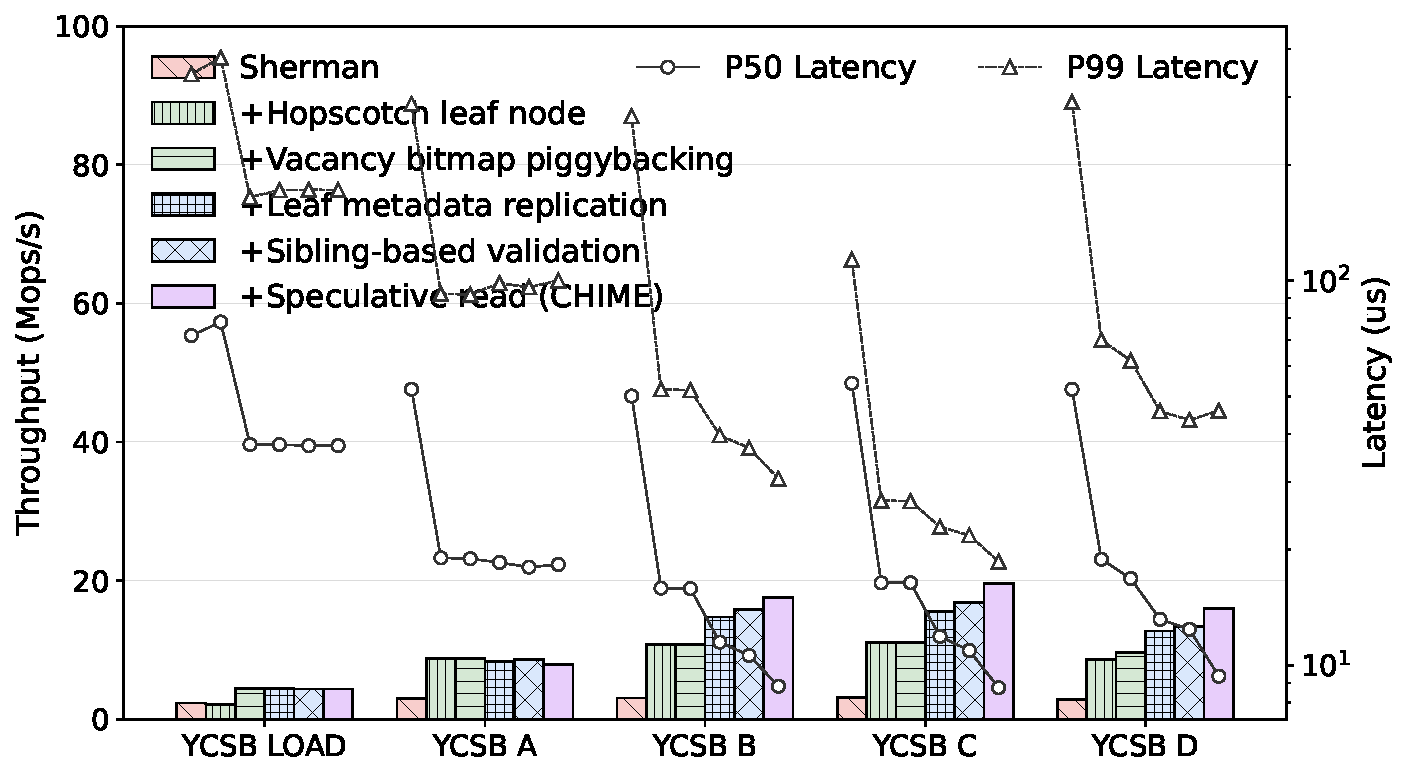
\includegraphics[width=0.95\textwidth]{figures/fig_15a.pdf}%
}{%
  
\includegraphics[width=0.95\textwidth]{../exp/results/fig_15a.pdf}%
}
\note{
  \textbf{Key point:} Each CHIME technique adds measurable throughput.\\
  \textbf{Say:} Here's our actual r650 data for Fig 15a---the Sherman-to-CHIME
  ablation. Each bar adds one technique. Hopscotch leaves give the biggest jump---
  3x on reads. Metadata replication adds another 50\% on read-heavy workloads.
  Speculative leaf read tops it off for YCSB B and C. The pattern matches
  the paper's claims closely.\\
  \textbf{Transition:} We also have the ROLEX ablation.\\
  \textbf{Time:} 50s
}
\end{frame}

% Slide 20 — Ablation Results (fig_15b)
\begin{frame}{Result: ROLEX $\to$ CHIME Ablation (r650)}
\centering
\IfFileExists{figures/fig_15b.pdf}{%
  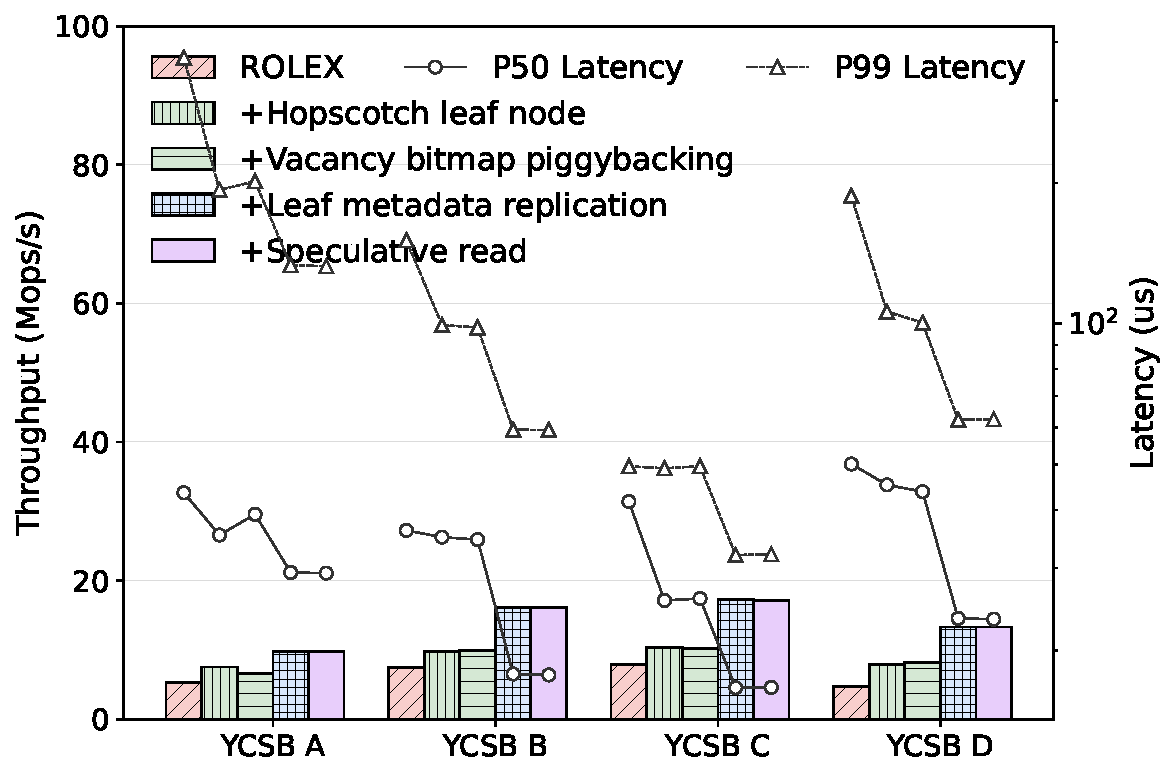
\includegraphics[width=0.95\textwidth]{figures/fig_15b.pdf}%
}{%
  
\includegraphics[width=0.95\textwidth]{../exp/results/fig_15b.pdf}%
}
\note{
  \textbf{Key point:} CHIME techniques also improve the learned index baseline.\\
  \textbf{Say:} Fig 15b starts from ROLEX---the learned index---and adds
  CHIME's techniques incrementally. Metadata replication is the biggest win
  here, nearly doubling throughput on read-heavy workloads. This confirms
  the techniques are general, not specific to the B+ tree baseline.\\
  \textbf{Transition:} And our throughput-latency data.\\
  \textbf{Time:} 45s
}
\end{frame}

% Slide 21 — Throughput-Latency (fig_12_c)
\begin{frame}{Result: Throughput vs Latency --- YCSB C (r650)}
\centering
\IfFileExists{figures/fig_12_c.pdf}{%
  \includegraphics[width=0.9\textwidth]{figures/fig_12_c.pdf}%
}{%
  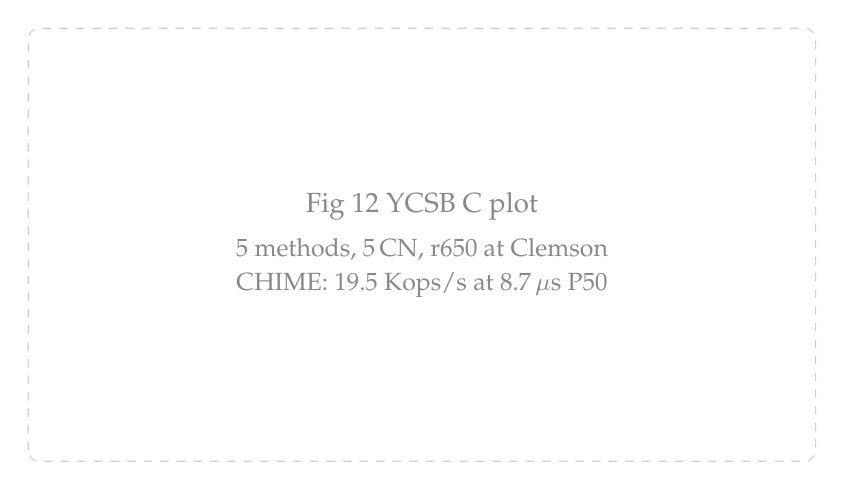
\begin{tikzpicture}
    \draw[mGray!40, dashed, rounded corners=4pt] (0,0) rectangle (10,5.5);
    \node[mGray, align=center, font=\normalsize] at (5,2.75)
      {Fig~12 YCSB~C plot\\[0.4em]
       {\small 5 methods, 5\,CN, r650 at Clemson}\\
       {\small CHIME: 19.5 Kops/s at 8.7\,$\mu$s P50}};
  \end{tikzpicture}%
}
\note{
  \textbf{Key point:} CHIME dominates on read-only workload.\\
  \textbf{Say:} YCSB C is 100\% reads. CHIME reaches 19.5 thousand ops
  per second with only 8.7 microseconds P50 latency---roughly 2.5x Sherman
  and 1.7x ROLEX. The speculative leaf read really shines here because every
  operation benefits from the hotspot buffer. Note we're running 5 compute
  nodes, not the paper's 10, so absolute throughput is lower but the
  relative ordering matches.\\
  \textbf{Transition:} Let's look at what's next---our CXL plan.\\
  \textbf{Time:} 50s
}
\end{frame}

\section{Backup: CXL Engineering Detail}

% Slide 20 — Why CXL?
\begin{frame}{RDMA vs.\ CXL}
\centering
\includegraphics[height=0.82\textheight]{diagrams/rdma-vs-cxl.pdf}
\note{
  \textbf{Key point:} CXL replaces NIC-mediated RDMA with direct load/store.\\
  \textbf{Say:} Part Two ports CHIME to CXL. CXL is the industry's answer
  to disaggregated memory---instead of going through a NIC with RDMA verbs,
  you do direct load/store to remote memory with hardware cache coherence.
  It's lower latency but changes the programming model fundamentally.\\
  \textbf{Transition:} Here's our porting approach.\\
  \textbf{Time:} 45s
}
\end{frame}

% Slide 21 — Transport Abstraction
\begin{frame}{Transport Abstraction Layer}
\centering
\includegraphics[height=0.82\textheight]{diagrams/transport-layer.pdf}
\note{
  \textbf{Key point:} Compile-time abstraction, zero overhead.\\
  \textbf{Say:} Our approach: a compile-time transport abstraction. The
  index code calls generic read/write/CAS operations. At build time, we
  select either the RDMA backend---which wraps the existing DSM---or
  the CXL backend, which uses NUMA-mapped memory with direct CPU
  operations. Zero vtable overhead thanks to C++ templates.\\
  \textbf{Transition:} How do we emulate CXL without real hardware?\\
  \textbf{Time:} 45s
}
\end{frame}

% Slide 22 — NUMA Emulation
\begin{frame}{NUMA Emulation on r650}
\centering
\includegraphics[height=0.82\textheight]{diagrams/numa-emulation.pdf}
\note{
  \textbf{Key point:} NUMA node 1 emulates CXL memory.\\
  \textbf{Say:} We don't have real CXL hardware, so we emulate it using
  the r650's second NUMA domain. Application threads run on socket 0,
  memory pool is bound to socket 1. Cross-socket latency approximates
  CXL's expected 100 to 200 nanoseconds of additional latency.\\
  \textbf{Transition:} What do we expect to find?\\
  \textbf{Time:} 40s
}
\end{frame}

% Slide 23 — What We Expect from CXL
\begin{frame}{CXL Hypotheses}
\centering
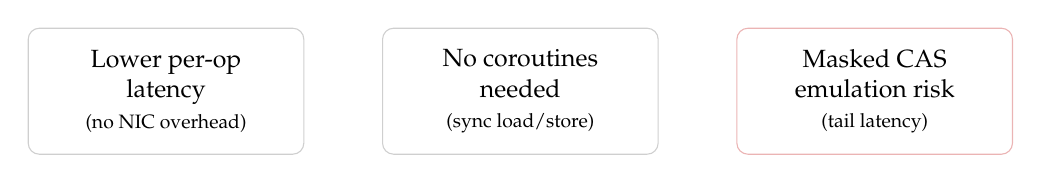
\begin{tikzpicture}[
  card/.style={draw=mGray!40, rounded corners=4pt, minimum width=3.5cm,
               minimum height=1.6cm, align=center, font=\small},
]
  \node[card] at (-4.5,0) {
    Lower per-op\\latency\\
    {\scriptsize(no NIC overhead)}
  };
  \node[card] at (0,0) {
    No coroutines\\needed\\
    {\scriptsize(sync load/store)}
  };
  \node[card, draw=mRed!40] at (4.5,0) {
    Masked CAS\\emulation risk\\
    {\scriptsize(tail latency)}
  };
\end{tikzpicture}
\note{
  \textbf{Key point:} Three hypotheses for the CXL port.\\
  \textbf{Say:} Three hypotheses. One: CXL should have lower per-operation
  latency---no NIC overhead. Two: RDMA uses coroutines to hide network
  latency; CXL doesn't need them because operations complete synchronously.
  Three: RDMA NICs support masked CAS natively, but CPUs don't---we'll
  need to emulate it, which could hurt tail latency under contention.\\
  \textbf{Transition:} Here's our timeline.\\
  \textbf{Time:} 45s
}
\end{frame}

% Slide 24 — CXL Engineering Completed
\begin{frame}{CXL Engineering: What We Built}
\small
\begin{tabular}{@{}p{0.42\textwidth}p{0.52\textwidth}@{}}
\toprule
\textbf{Artifact} & \textbf{Status} \\
\midrule
\texttt{CxlTransport} / \texttt{CxlDSM}        & Single-flag transport swap (\texttt{USE\_CXL=ON}) \\
\texttt{Dockerfile.cxl-preflight}              & Reproducible build from clone \\
5-blocker fix sequence (\texttt{152b4e9}$\to$\texttt{e430d8d}) & All blockers closed in Docker \\
\texttt{exp/run\_harness.py}                   & Debug capture on failure (8/8 tests) \\
\texttt{exp/fig\_14\_surrogate.py}             & 60M-key cache surrogate (5/5 tests) \\
\texttt{exp/plot\_fig\_12\_three\_way.py}      & 3-way comparison plotter (5/5 tests) \\
\texttt{smoke-gate.sh}                         & 5\,s LOAD + 30\,s YCSB C automated gate \\
\texttt{runbook-day1.md}                       & T+0:00 to T+7:30 hardware-window playbook \\
\bottomrule
\end{tabular}
\vspace{0.3em}
\centering\small
{\color{mGreen}\textbf{18 unit tests passing, builds clean, reproducible from clone.}}
\note{
  \textbf{Key point:} Engineering side of Part Two is fully done.\\
  \textbf{Say:} Everything we could build off-hardware, we built and tested. The transport port itself, the Docker preflight that catches build regressions in two minutes of CI, the harness that auto-captures debug artifacts on any failure, a single-point cache-consumption surrogate, the three-way plot helper, and an automated smoke gate that defines what "the CXL port works" means in 35 seconds of cluster time. Eighteen unit tests pass. Reproduces from clone via Docker. None of this depends on a successful runtime evaluation.\\
  \textbf{Transition:} What we couldn't do is run any of it on r650.\\
  \textbf{Time:} 60s
}
\end{frame}

\section{Backup: Additional Runtime Data}

\begin{frame}{CXL vs RDMA: 17 New Data Points}
\centering
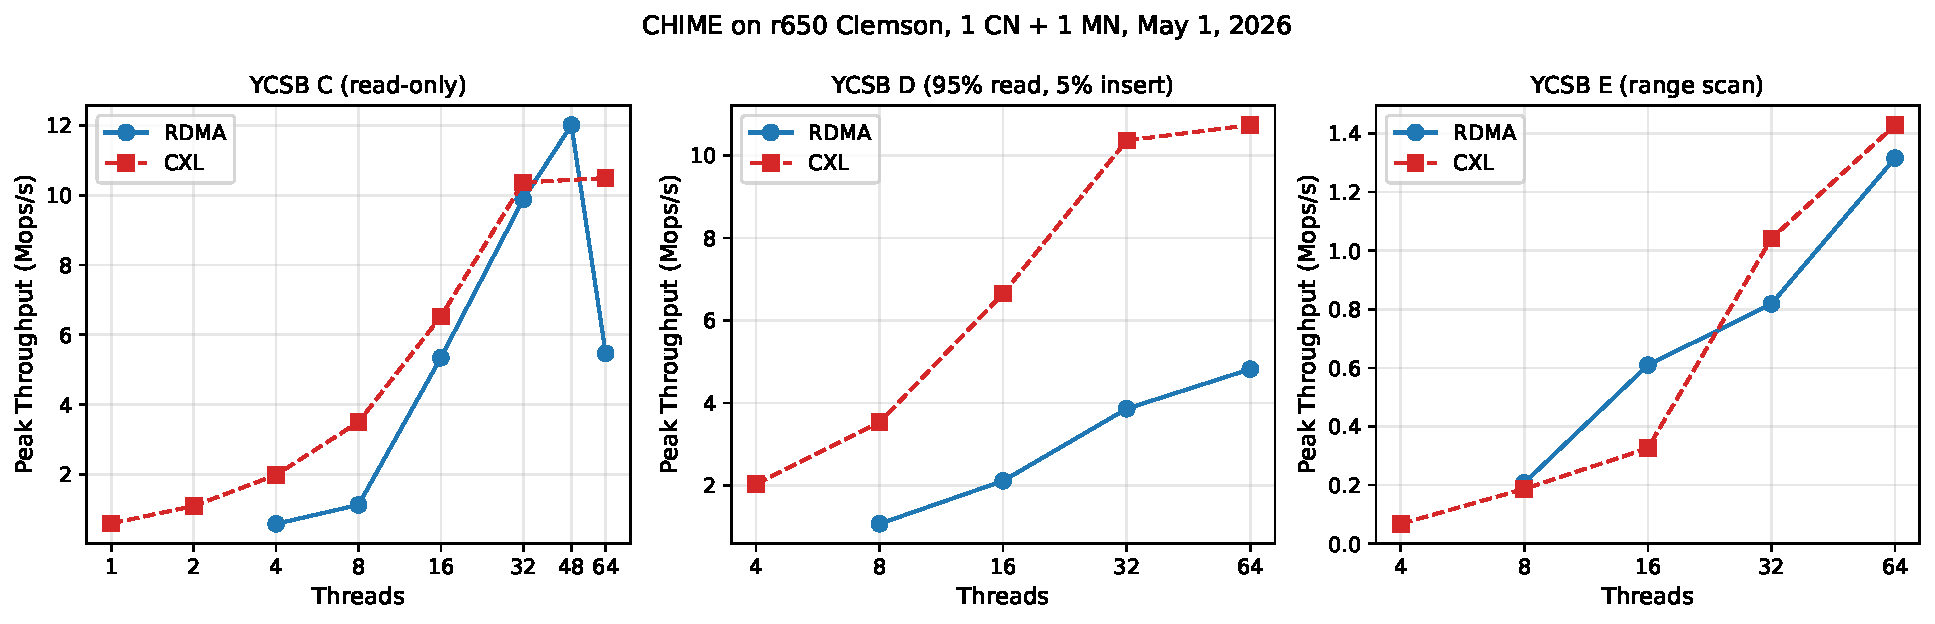
\includegraphics[height=0.78\textheight]{../report/figures/fig12-rdma-vs-cxl.pdf}
\note{
  \textbf{Key point:} CXL wins on read-heavy workloads, loses on range scans at low thread counts.\\
  \textbf{Say:} Three panels, three workloads. C is read-only, D is 95\% read 5\% insert, E is range scan. CXL in red, RDMA in blue. On C and D, CXL roughly triples RDMA's throughput at low to mid thread counts. The picture flips on E. Range scans benefit from RDMA's coroutine-pipelined reads. CXL is synchronous --- each memcpy blocks. So at 16 threads CXL is half RDMA on E. Above 32 threads thread parallelism makes up for the missing intra-thread pipelining and CXL catches up.\\
  \textbf{Transition:} The speedup ratio makes the workload-dependence clearer.\\
  \textbf{Time:} 80s
}
\end{frame}

\begin{frame}{Single-CN Competitors: Sherman, SMART, ROLEX}
\centering
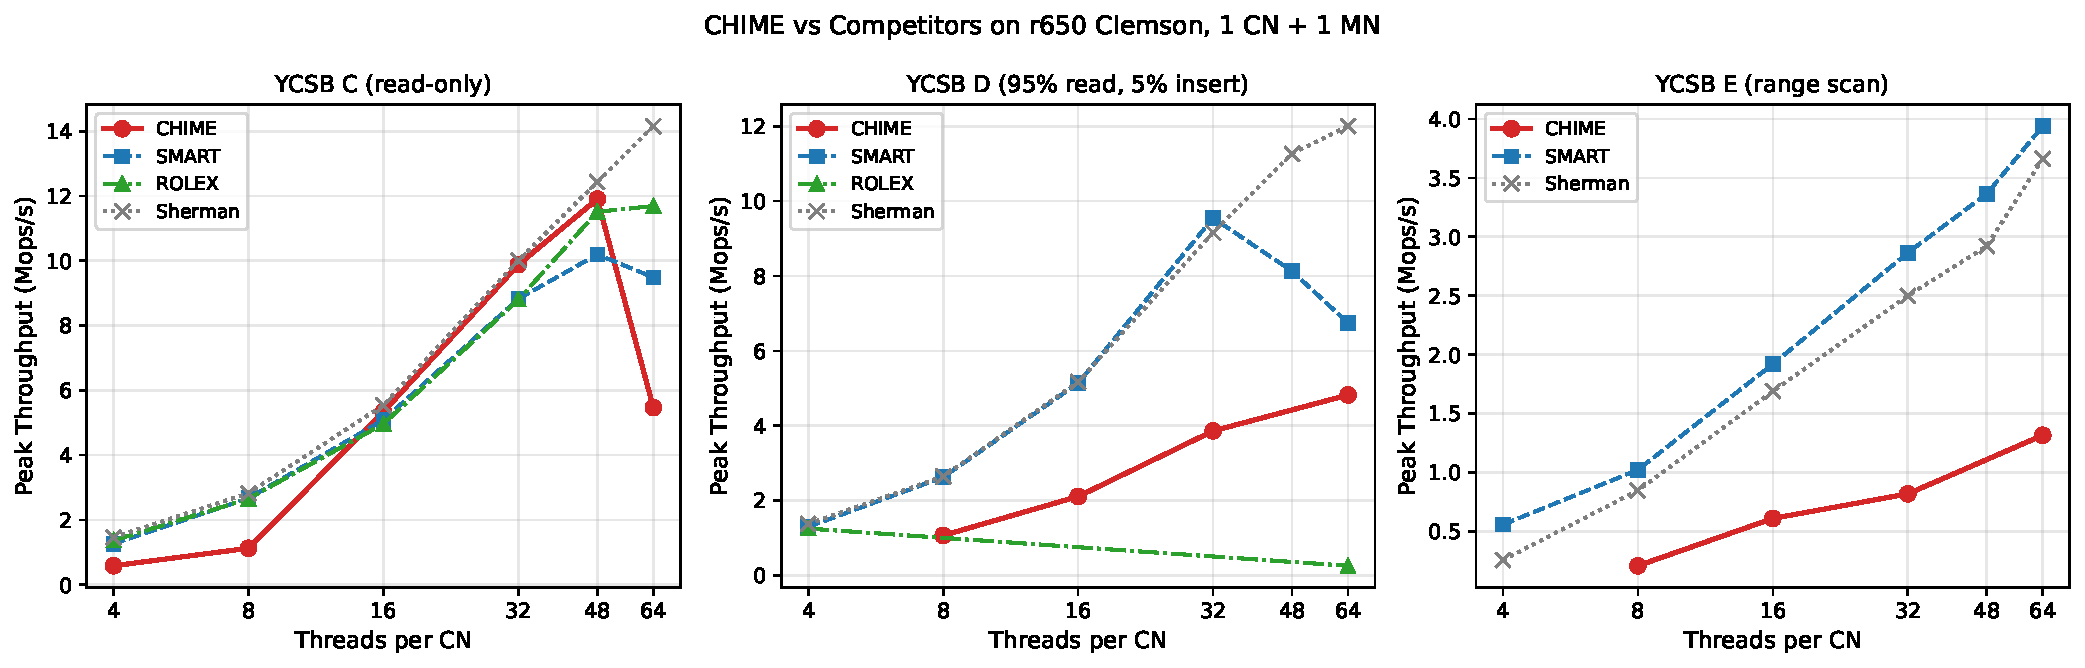
\includegraphics[height=0.78\textheight]{../report/figures/fig12-competitors.pdf}
\note{
  \textbf{Key point:} The May 2 cluster also gave us SMART, Sherman, and ROLEX on the same single-CN hardware --- so the competitor comparison is now apples-to-apples with our CXL data, not just the multi-CN runs.\\
  \textbf{Say:} The May 1 cluster stayed alive long enough to extend the comparison. We rebuilt CHIME with all five features off (that's Sherman) plus dropped in SMART from dmemsys/SMART and ROLEX from River861's CHIME-compatible re-implementation. All four methods share the same harness --- same memcached coordination, same workload files, same ycsb\_test entry point. Sherman scales most aggressively on C: 14 Mops/s at 64 threads, no per-operation overhead from CHIME's hopscotch displacement or speculative read. SMART peaks at 10 then regresses --- its update-in-place leaves bottleneck at high concurrency. ROLEX shipped in time only for workload C; on D and E its 60-million pre-train key load plus learned-model training blew past our 90-second per-point budget. We re-ran ROLEX D with a 300-second budget after the main sweep.\\
  \textbf{Transition:} Three things stand out about this picture.\\
  \textbf{Time:} 75s
}
\end{frame}

\begin{frame}{What the Single-CN Competitor Curves Tell Us}
\small
\textbf{Three findings} from the May 2 single-CN sweep:
\begin{itemize}
  \item \textbf{Curve shapes match the paper.} Sherman scales linearly on C to 64 threads; CHIME / SMART / ROLEX bend earlier --- same shape as the paper's Figure~12, shifted down by the single-CN factor.
  \item \textbf{ROLEX's training cost is real.} 60\,M pre-train keys $+$ epsilon-bounded model fitting, all serialized on the CN. Easy to miss in the paper's reporting; surfaced here as an operational consideration for learned indexes on disaggregated memory.
  \item \textbf{Methods cluster on a single CN.} Gap is at most $1.4\times$ on C, $1.3\times$ on D, $1.1\times$ on E. The paper's wider gaps appear at multi-CN scale --- consistent with coordination overhead amortizing differently as CN count grows.
\end{itemize}
\end{frame}

\begin{frame}{Sherman-on-CXL: Isolating Transport from Features}
\centering
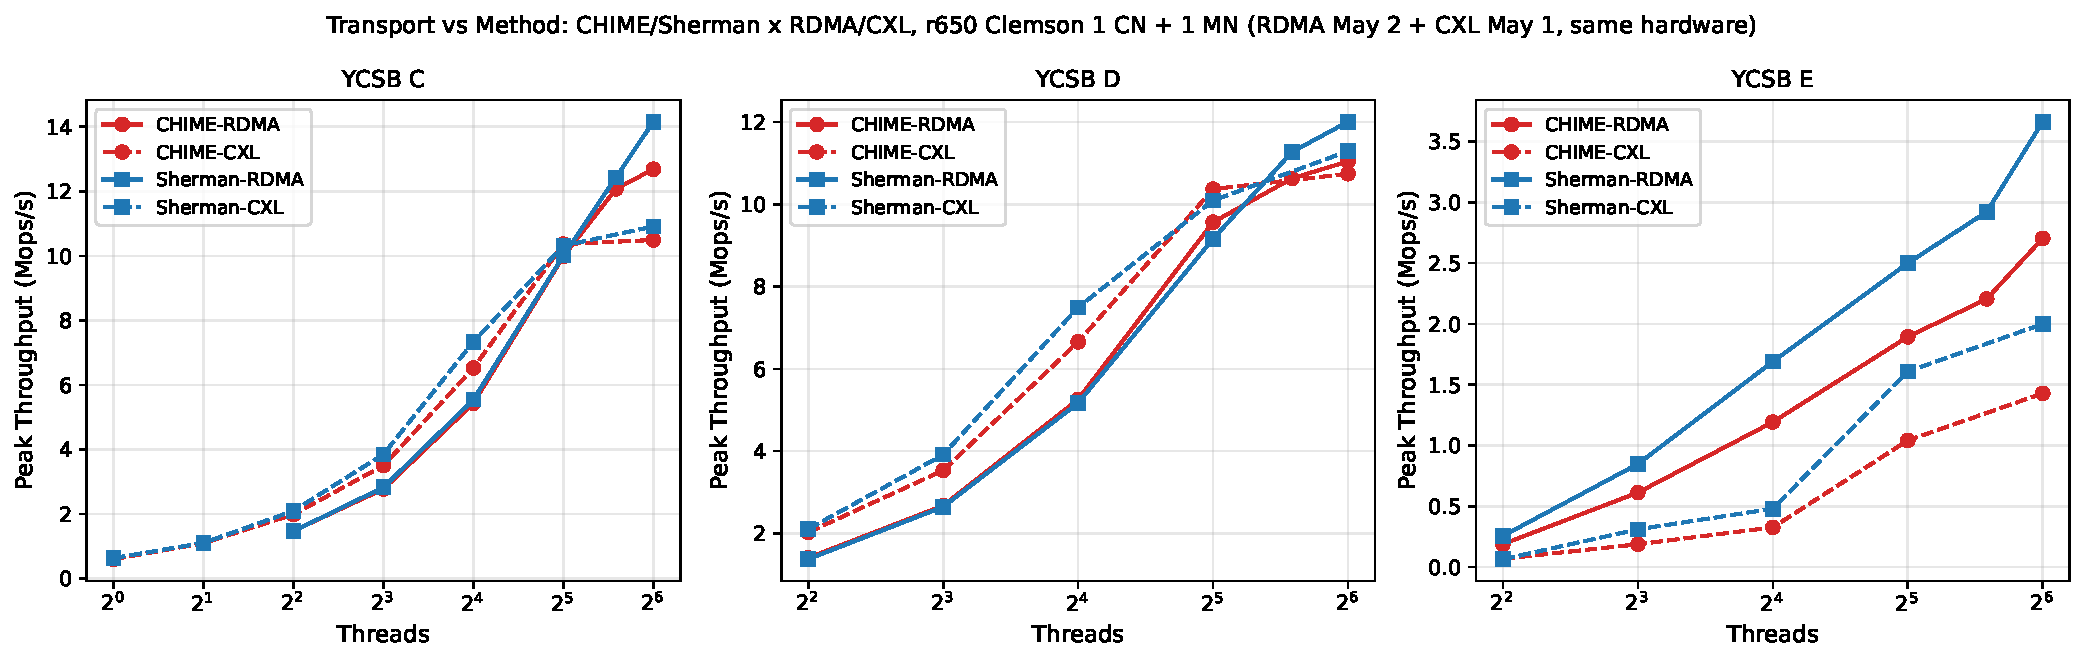
\includegraphics[height=0.65\textheight]{../report/figures/fig12-transport-method.pdf}
\note{
  \textbf{Key point:} Building Sherman with USE\_CXL=on (Sherman is just CHIME's source with all 5 features off) lets us separate the transport benefit from the feature benefit.\\
  \textbf{Say:} Sherman is built from CHIME's source tree with all five feature flags compiled out, so it shares CHIME's CXL transport. The 2x2 chart isolates "what does CXL transport buy you" from "what do CHIME's features add on top." Pattern is consistent: CXL beats RDMA on C and D for both methods, loses badly on E for both methods. CXL gives Sherman about a 1.4x speedup on C at low threads, similar to CHIME's same-day CXL/RDMA ratio. So the CXL win on this hardware is mostly transport-driven --- the lower latency of NUMA-loop reads versus a 2-microsecond RDMA round trip --- and mostly independent of CHIME's feature stack on the workloads where CXL wins.\\
  \textbf{Transition:} The bigger surprise was the cross-day RDMA variance.\\
  \textbf{Time:} 60s
}
\end{frame}

\section{Backup: Postmortem Timeline}

% Slide — Reservation Outage Timeline
\begin{frame}{The Reservation Outage}
\small
Four r650 Clemson reservations against project \texttt{CS620426SP}, April 22--26:
\vspace{0.3em}
\begin{center}
\begin{tabular}{@{}llll@{}}
\toprule
Window & UUID (truncated) & Hardware & Outcome \\
\midrule
Apr 22, 8h auto              & \texttt{43677ece}\ldots & 2$\times$r650 & Expired unused \\
Apr 23, 8h auto              & \texttt{5565ec96}\ldots & 2$\times$r650 & {\color{mRed}Failed} \\
Apr 20--25, 5d admin         & \texttt{8c36e934}\ldots & 2$\times$r650 & {\color{mRed}Failed} \\
Apr 21--26, 5d admin         & \texttt{cc0bf3c0}\ldots & 2$\times$r650 & {\color{mRed}Failed} \\
Apr 27, 1d auto              & \texttt{2afbcb47}\ldots & 2$\times$r650 & {\color{mGreen}Honored} \\
\bottomrule
\end{tabular}
\end{center}
\vspace{0.5em}
\textbf{80+ hours of approved capacity. Zero nodes ever provisioned.}
\note{
  \textbf{Key point:} Four reservations, none honored.\\
  \textbf{Say:} Four reservations, totaling more than 80 hours of approved capacity. The April 22 window we lost ourselves --- pre-hardware tooling overran the start. The other three were CloudLab. Every single startExperiment against an active reservation failed within ninety seconds with the same error.\\
  \textbf{Transition:} Here is that error, verbatim.\\
  \textbf{Time:} 45s
}
\end{frame}

\section{Backup: Late Data Supplements}

\begin{frame}[fragile]{What We Got on the r650 Reservation}
\small After fixing three ConnectX-6 Dx compatibility issues (\texttt{MAX\_ATOMIC\_ARG=8}, \texttt{max\_recv\_sge=2 for UD}, \texttt{openibd restart} to populate \texttt{device\_cap\_flags}):
\vspace{0.3em}
\begin{center}
\textbf{fig\_12 Throughput-Thread Curves, 1\,CN $+$ 1\,MN, peak Mops/s} \\[0.3em]
\begin{tabular}{@{}rrrr@{}}
\toprule
Threads & C (read-only) & D (95\%R/5\%I) & E (range scan) \\
\midrule
8   & 1.12          & 1.07           & 0.21          \\
16  & 3.26 (n=3)$\dagger$ & 2.11    & 0.61          \\
32  & 4.21 (n=3)    & 3.86           & 0.82          \\
48  & 5.19 (n=3)    & ---            & ---           \\
64  & 5.36 (n=3)    & 4.82           & 1.32          \\
\bottomrule
\end{tabular}
\end{center}
\vspace{0.3em}
{\scriptsize $\dagger$ Bimodal across 8--10 reps: $\sim$2 of 10 runs land on the warm-cache mode ($\sim$5.34); the rest sit at $\sim$2.22 --- hotspot buffer warm/cold transition}
\note{
  \textbf{Key point:} Real fig\_12 data — 12+ runs, 3 workloads, 4 thread counts.\\
  \textbf{Say:} The April 27 reservation finally went through after we fixed three Dx compatibility issues. We got a complete throughput-thread curve for YCSB C, D, and E on a single CN single MN config. C is read-only and shows the cleanest scaling. D scales similarly. E is much slower because range scans are expensive. The 16-thread bimodality on C is interesting — across roughly ten reps, two runs land on the warm-cache mode at 5.3 Mops and the rest sit at the cold-cache 2.2 Mops floor. The transition is sharp because at 16 threads the hotspot buffer either warms up before the measurement epoch starts or it doesn't.\\
  \textbf{Transition:} We also ran the per-technique ablation.\\
  \textbf{Time:} 70s
}
\end{frame}

\begin{frame}{fig\_15a Ablation: Sherman \texttt{->} CHIME on YCSB C/D}
\small Cumulative ablation, 16 (C) or 32 (D) threads, peak Mops/s:
\vspace{0.3em}
\begin{center}
\begin{tabular}{@{}lrr@{}}
\toprule
Variant & C (16t) & D (32t) \\
\midrule
Sherman-equivalent (all OFF)             & {\color{mRed}build failed} & --- \\
$+$ \texttt{HOPSCOTCH\_LEAF\_NODE}       & 2.14 & 3.76 \\
$+$ \texttt{VACANCY\_AWARE\_LOCK}        & 2.15 & 3.75 \\
$+$ \texttt{METADATA\_REPLICATION}       & {\color{mGreen}\textbf{2.40}} & {\color{mGreen}\textbf{4.16}} \\
$+$ \texttt{SIBLING\_BASED\_VALIDATION}  & 2.40 & 4.13 \\
$+$ \texttt{SPECULATIVE\_READ} (full)    & 2.22 & 3.89 \\
\bottomrule
\end{tabular}
\end{center}
\vspace{0.3em}
\textbf{Findings:}
\begin{itemize}[nosep]
    \item \texttt{METADATA\_REPLICATION} is the only single-CN winner (saves an RTT per metadata read).
    \item \texttt{VACANCY\_AWARE\_LOCK}, \texttt{SIBLING\_BASED\_VALIDATION}: no-ops on perf at 1\,CN; they're correctness mechanisms (Sherman LOAD finding).
    \item \texttt{SPECULATIVE\_READ} is slightly negative without cross-CN access patterns.
    \item Sherman-equivalent build (all features OFF) does not link --- artifact-buildability finding.
\end{itemize}
\note{
  \textbf{Key point:} Per-technique deltas at 1 CN reveal which techniques need cross-CN coordination.\\
  \textbf{Say:} We ran the same six-variant cumulative ablation that the paper does for fig 15a, but at one CN instead of ten. Only metadata replication moves the needle. Vacancy-aware lock is a no-op because there's no cross-CN write contention. Sibling-based validation is a correctness mechanism — it doesn't add throughput, it prevents the Sherman crash. Speculative read is slightly negative because the hotspot buffer relies on access patterns that single-CN can't produce. The all-features-OFF build doesn't link, which is itself an artifact-paper finding.\\
  \textbf{Transition:} The CXL port hit a wall in the worker thread.\\
  \textbf{Time:} 70s
}
\end{frame}

% Slide — Future Work
\begin{frame}{Future Work}
\small Hardware time, reasoned about as cost-of-experiment:
\vspace{0.3em}
\begin{itemize}[nosep]
    \item \textbf{Smoke gate first.} The first datum --- pass/fail on 5\,s LOAD + 30\,s YCSB C --- is more informative than any speculation in this deck.
    \item \textbf{Single-CN fig\_12 sweep on CXL.} If the gate passes, this is the central evaluation artifact (~3 hours).
    \item \textbf{RDMA single-node baseline + per-thread regression check.} Validates the transport refactor didn't silently break RDMA (~1.5 hours).
    \item \textbf{fig\_15a/b ablation on CXL.} Per-technique deltas tell us which optimizations remain load-bearing when transport latency drops 10$\times$ (~1.5 hours).
    \item \textbf{Sibling-method CXL ports} (Sherman, SMART, ROLEX, Marlin). Each requires its own transport substitution, not all are 5-blocker series.
    \item \textbf{Real CXL hardware.} Adds protocol-credit accounting that NUMA emulation does not model.
\end{itemize}
\note{
  \textbf{Key point:} Concrete future work, ordered by information value per cluster hour.\\
  \textbf{Say:} If a reservation opens up, here's the order of operations. Smoke gate first --- 35 seconds tells you whether the port runs at all. fig\_12 on CHIME-CXL is the central artifact. The RDMA single-node baseline plus a per-thread regression check confirms the refactor didn't silently break RDMA. The ablation tells us which optimizations still pay off when latency drops by an order of magnitude. Then sibling ports, then real CXL.\\
  \textbf{Transition:} Three takeaways.\\
  \textbf{Time:} 50s
}
\end{frame}

\section{Backup: Q\&A and References}

% Slide — Questions (first; References follows for Q&A backup)
{
\setbeamercolor{background canvas}{bg=myRed}
\begin{frame}[plain]
\vspace*{\fill}
\begin{center}
{\color{white}\Huge\bfseries Questions?}
\end{center}
\vspace*{\fill}
\note{
  \textbf{Key point:} Open floor.\\
  \textbf{Say:} Thank you. Happy to take questions about the reproduction,
  our CXL plans, or anything about CHIME's design.\\
  \textbf{Transition:} ---\\
  \textbf{Time:} remainder
}
\end{frame}
}

% Slide — References (after Questions; reachable for Q&A citations)
\begin{frame}[allowframebreaks]{References}
\begin{thebibliography}{9}
\footnotesize

\bibitem{chime2024}
X.~Luo, J.~Shen, P.~Zuo, X.~Wang, M.~R.~Lyu, Y.~Zhou.
\newblock {CHIME}: A Cache-Efficient and High-Performance Hybrid Index on Disaggregated Memory.
\newblock \emph{SOSP}, 2024.

\bibitem{sherman2022}
Q.~Wang, Y.~Lu, J.~Shu.
\newblock {Sherman}: A Write-Optimized Distributed {B+Tree} Index on Disaggregated Memory.
\newblock \emph{SIGMETRICS}, 2022.

\bibitem{smart2023}
X.~Luo, P.~Zuo, J.~Shen, J.~Zhou, Y.~Zhou.
\newblock {SMART}: A High-Performance Adaptive Radix Tree for Disaggregated Memory.
\newblock \emph{USENIX ATC}, 2023.

\bibitem{rolex2024}
P.~Li, Y.~Hua, J.~Chen, J.~Zhang.
\newblock {ROLEX}: A Scalable {RDMA}-optimized Learned Key-Value Store for Disaggregated Memory Systems.
\newblock \emph{USENIX FAST}, 2023.

\bibitem{cxl}
CXL Consortium.
\newblock Compute Express Link Specification, Rev.~3.1.
\newblock 2024.

\bibitem{ornl-agents-xloop25}
D.~Rosendo, S.~DeWitt, R.~Souza, P.~Austria, T.~Ghosal, M.~McDonnell,
R.~Miller, T.~J.~Skluzacek, J.~Haley, B.~Turcksin, J.~McGaha, B.~Mintz,
F.~Wang, M.~Shankar, S.~Oral, R.~Ferreira~da~Silva.
\newblock {AI} Agents for Enabling Autonomous Experiments at {ORNL}'s {HPC}
and Manufacturing User Facilities.
\newblock \emph{XLOOP '25 (SC '25 Workshops)}, 2025.

\end{thebibliography}
\note{
  \textbf{Key point:} Reference slide.\\
  \textbf{Say:} (No spoken content---reference slide for Q\&A.)\\
  \textbf{Transition:} ---\\
  \textbf{Time:} 5s
}
\end{frame}

\end{document}
